\subsubsection{Resultados}
\par Se presentan a continuaci\'on los resultados de la experimentaci\'on
    de la heur\'istica de b\'usqueda local para \emph{CMF}. La experimentaci\'on se realiz\'o
    con las instancias ya generadas (seg\'un se explica en \emph{\nameref{notas_preliminares},
    \nameref{notas:datasets}} y \emph{\nameref{notas:experimentacion}}).

\par Para recordar, se cuentan con 10 instancias aleatorias de cada tama\~no,
    las cuales fueron resueltas 5 veces cada una y nos quedamos con el menor tiempo
    requerido de esas 5 ejecuciones. Por \'ultimo, tomamos el promedio de este tiempo
    requerido calculado entre las instancias del mismo tama\~no (10, como se ha
    dicho).

\par En los gr\'aficos que se muestran a continuaci\'on, se aprovech\'o el hecho
    de que la complejidad te\'orica de esta heur\'istica y sus variantes fuera
    polinomial. Lo que se hizo luego de realizar la experimentaci\'on, fue
    tomar las mediciones y aplicarles la ra\'iz correspondiente (para la heur\'istica
    sin intercambio ser\'a la ra\'iz cuarta y con intercambio la ra\'iz quinta).

\par De esta manera, linealizamos las complejidades emp\'iricas, los cual nos permite
    comparar dichas mediciones en el plano con una funci\'on $\mathcal O(n)$, haciendo
    m\'as f\'acil la comparaci\'on visual.

\bigskip

\begin{figure}[H]
    \centering
    \fontsize{7}{10}\selectfont
    \resizebox{0.8\textwidth}{!}{% GNUPLOT: LaTeX picture with Postscript
\begingroup
  \makeatletter
  \providecommand\color[2][]{%
    \GenericError{(gnuplot) \space\space\space\@spaces}{%
      Package color not loaded in conjunction with
      terminal option `colourtext'%
    }{See the gnuplot documentation for explanation.%
    }{Either use 'blacktext' in gnuplot or load the package
      color.sty in LaTeX.}%
    \renewcommand\color[2][]{}%
  }%
  \providecommand\includegraphics[2][]{%
    \GenericError{(gnuplot) \space\space\space\@spaces}{%
      Package graphicx or graphics not loaded%
    }{See the gnuplot documentation for explanation.%
    }{The gnuplot epslatex terminal needs graphicx.sty or graphics.sty.}%
    \renewcommand\includegraphics[2][]{}%
  }%
  \providecommand\rotatebox[2]{#2}%
  \@ifundefined{ifGPcolor}{%
    \newif\ifGPcolor
    \GPcolortrue
  }{}%
  \@ifundefined{ifGPblacktext}{%
    \newif\ifGPblacktext
    \GPblacktexttrue
  }{}%
  % define a \g@addto@macro without @ in the name:
  \let\gplgaddtomacro\g@addto@macro
  % define empty templates for all commands taking text:
  \gdef\gplbacktext{}%
  \gdef\gplfronttext{}%
  \makeatother
  \ifGPblacktext
    % no textcolor at all
    \def\colorrgb#1{}%
    \def\colorgray#1{}%
  \else
    % gray or color?
    \ifGPcolor
      \def\colorrgb#1{\color[rgb]{#1}}%
      \def\colorgray#1{\color[gray]{#1}}%
      \expandafter\def\csname LTw\endcsname{\color{white}}%
      \expandafter\def\csname LTb\endcsname{\color{black}}%
      \expandafter\def\csname LTa\endcsname{\color{black}}%
      \expandafter\def\csname LT0\endcsname{\color[rgb]{1,0,0}}%
      \expandafter\def\csname LT1\endcsname{\color[rgb]{0,1,0}}%
      \expandafter\def\csname LT2\endcsname{\color[rgb]{0,0,1}}%
      \expandafter\def\csname LT3\endcsname{\color[rgb]{1,0,1}}%
      \expandafter\def\csname LT4\endcsname{\color[rgb]{0,1,1}}%
      \expandafter\def\csname LT5\endcsname{\color[rgb]{1,1,0}}%
      \expandafter\def\csname LT6\endcsname{\color[rgb]{0,0,0}}%
      \expandafter\def\csname LT7\endcsname{\color[rgb]{1,0.3,0}}%
      \expandafter\def\csname LT8\endcsname{\color[rgb]{0.5,0.5,0.5}}%
    \else
      % gray
      \def\colorrgb#1{\color{black}}%
      \def\colorgray#1{\color[gray]{#1}}%
      \expandafter\def\csname LTw\endcsname{\color{white}}%
      \expandafter\def\csname LTb\endcsname{\color{black}}%
      \expandafter\def\csname LTa\endcsname{\color{black}}%
      \expandafter\def\csname LT0\endcsname{\color{black}}%
      \expandafter\def\csname LT1\endcsname{\color{black}}%
      \expandafter\def\csname LT2\endcsname{\color{black}}%
      \expandafter\def\csname LT3\endcsname{\color{black}}%
      \expandafter\def\csname LT4\endcsname{\color{black}}%
      \expandafter\def\csname LT5\endcsname{\color{black}}%
      \expandafter\def\csname LT6\endcsname{\color{black}}%
      \expandafter\def\csname LT7\endcsname{\color{black}}%
      \expandafter\def\csname LT8\endcsname{\color{black}}%
    \fi
  \fi
  \setlength{\unitlength}{0.0500bp}%
  \begin{picture}(7200.00,5040.00)%
    \gplgaddtomacro\gplbacktext{%
      \csname LTb\endcsname%
      \put(1034,1375){\makebox(0,0)[r]{\strut{} 10}}%
      \csname LTb\endcsname%
      \put(1034,1875){\makebox(0,0)[r]{\strut{} 20}}%
      \csname LTb\endcsname%
      \put(1034,2376){\makebox(0,0)[r]{\strut{} 30}}%
      \csname LTb\endcsname%
      \put(1034,2877){\makebox(0,0)[r]{\strut{} 40}}%
      \csname LTb\endcsname%
      \put(1034,3378){\makebox(0,0)[r]{\strut{} 50}}%
      \csname LTb\endcsname%
      \put(1034,3878){\makebox(0,0)[r]{\strut{} 60}}%
      \csname LTb\endcsname%
      \put(1034,4379){\makebox(0,0)[r]{\strut{} 70}}%
      \csname LTb\endcsname%
      \put(1165,704){\makebox(0,0){\strut{} 0}}%
      \csname LTb\endcsname%
      \put(1729,704){\makebox(0,0){\strut{} 500}}%
      \csname LTb\endcsname%
      \put(2292,704){\makebox(0,0){\strut{} 1000}}%
      \csname LTb\endcsname%
      \put(2856,704){\makebox(0,0){\strut{} 1500}}%
      \csname LTb\endcsname%
      \put(3420,704){\makebox(0,0){\strut{} 2000}}%
      \csname LTb\endcsname%
      \put(3984,704){\makebox(0,0){\strut{} 2500}}%
      \csname LTb\endcsname%
      \put(4548,704){\makebox(0,0){\strut{} 3000}}%
      \csname LTb\endcsname%
      \put(5112,704){\makebox(0,0){\strut{} 3500}}%
      \csname LTb\endcsname%
      \put(5675,704){\makebox(0,0){\strut{} 4000}}%
      \csname LTb\endcsname%
      \put(6239,704){\makebox(0,0){\strut{} 4500}}%
      \csname LTb\endcsname%
      \put(6803,704){\makebox(0,0){\strut{} 5000}}%
      \put(176,2651){\rotatebox{-270}{\makebox(0,0){\strut{}Tiempo ($microsegundos^{\sfrac{1}{5}}$)}}}%
      \put(396,2651){\rotatebox{-270}{\makebox(0,0){\strut{}(Escala Lineal)}}}%
      \put(3984,374){\makebox(0,0){\strut{}Cantidad de Nodos}}%
      \put(3984,154){\makebox(0,0){\strut{}(Escala Lineal)}}%
      \put(3984,4709){\makebox(0,0){\strut{}Tiempo de ejecución conforme aumenta la cantidad de nodos}}%
    }%
    \gplgaddtomacro\gplfronttext{%
      \csname LTb\endcsname%
      \put(3928,4269){\makebox(0,0)[r]{\strut{}Primer Vecino}}%
      \csname LTb\endcsname%
      \put(3928,4049){\makebox(0,0)[r]{\strut{}Primer Vecino con golosa}}%
      \csname LTb\endcsname%
      \put(3928,3829){\makebox(0,0)[r]{\strut{}Primer Vecino con intercambio}}%
      \csname LTb\endcsname%
      \put(3928,3609){\makebox(0,0)[r]{\strut{}Primer Vecino con intercambio y golosa}}%
      \csname LTb\endcsname%
      \put(3928,3389){\makebox(0,0)[r]{\strut{}Mejor Vecino}}%
      \csname LTb\endcsname%
      \put(3928,3169){\makebox(0,0)[r]{\strut{}Mejor Vecino con golosa}}%
      \csname LTb\endcsname%
      \put(3928,2949){\makebox(0,0)[r]{\strut{}Mejor Vecino con intercambio}}%
      \csname LTb\endcsname%
      \put(3928,2729){\makebox(0,0)[r]{\strut{}Mejor Vecino con intercambio y golosa}}%
      \csname LTb\endcsname%
      \put(3928,2509){\makebox(0,0)[r]{\strut{}Cota teórica superior $\mathcal O(n)$}}%
    }%
    \gplbacktext
    \put(0,0){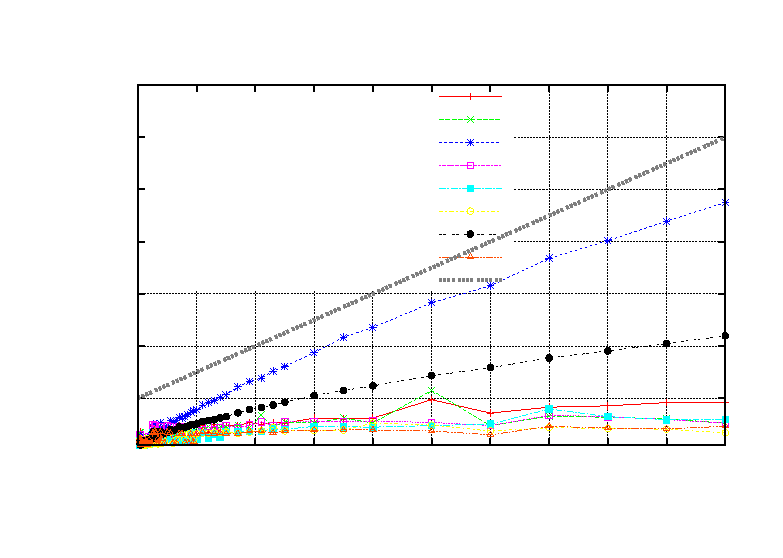
\includegraphics{ej3_nodos_star+cmf}}%
    \gplfronttext
  \end{picture}%
\endgroup
}
    \caption{Complejidad temporal para grafos Estrella+CMF}
\end{figure}

\begin{figure}[H]
    \centering
    \fontsize{7}{10}\selectfont
    \resizebox{0.87\textwidth}{!}{% GNUPLOT: LaTeX picture with Postscript
\begingroup
  \makeatletter
  \providecommand\color[2][]{%
    \GenericError{(gnuplot) \space\space\space\@spaces}{%
      Package color not loaded in conjunction with
      terminal option `colourtext'%
    }{See the gnuplot documentation for explanation.%
    }{Either use 'blacktext' in gnuplot or load the package
      color.sty in LaTeX.}%
    \renewcommand\color[2][]{}%
  }%
  \providecommand\includegraphics[2][]{%
    \GenericError{(gnuplot) \space\space\space\@spaces}{%
      Package graphicx or graphics not loaded%
    }{See the gnuplot documentation for explanation.%
    }{The gnuplot epslatex terminal needs graphicx.sty or graphics.sty.}%
    \renewcommand\includegraphics[2][]{}%
  }%
  \providecommand\rotatebox[2]{#2}%
  \@ifundefined{ifGPcolor}{%
    \newif\ifGPcolor
    \GPcolortrue
  }{}%
  \@ifundefined{ifGPblacktext}{%
    \newif\ifGPblacktext
    \GPblacktexttrue
  }{}%
  % define a \g@addto@macro without @ in the name:
  \let\gplgaddtomacro\g@addto@macro
  % define empty templates for all commands taking text:
  \gdef\gplbacktext{}%
  \gdef\gplfronttext{}%
  \makeatother
  \ifGPblacktext
    % no textcolor at all
    \def\colorrgb#1{}%
    \def\colorgray#1{}%
  \else
    % gray or color?
    \ifGPcolor
      \def\colorrgb#1{\color[rgb]{#1}}%
      \def\colorgray#1{\color[gray]{#1}}%
      \expandafter\def\csname LTw\endcsname{\color{white}}%
      \expandafter\def\csname LTb\endcsname{\color{black}}%
      \expandafter\def\csname LTa\endcsname{\color{black}}%
      \expandafter\def\csname LT0\endcsname{\color[rgb]{1,0,0}}%
      \expandafter\def\csname LT1\endcsname{\color[rgb]{0,1,0}}%
      \expandafter\def\csname LT2\endcsname{\color[rgb]{0,0,1}}%
      \expandafter\def\csname LT3\endcsname{\color[rgb]{1,0,1}}%
      \expandafter\def\csname LT4\endcsname{\color[rgb]{0,1,1}}%
      \expandafter\def\csname LT5\endcsname{\color[rgb]{1,1,0}}%
      \expandafter\def\csname LT6\endcsname{\color[rgb]{0,0,0}}%
      \expandafter\def\csname LT7\endcsname{\color[rgb]{1,0.3,0}}%
      \expandafter\def\csname LT8\endcsname{\color[rgb]{0.5,0.5,0.5}}%
    \else
      % gray
      \def\colorrgb#1{\color{black}}%
      \def\colorgray#1{\color[gray]{#1}}%
      \expandafter\def\csname LTw\endcsname{\color{white}}%
      \expandafter\def\csname LTb\endcsname{\color{black}}%
      \expandafter\def\csname LTa\endcsname{\color{black}}%
      \expandafter\def\csname LT0\endcsname{\color{black}}%
      \expandafter\def\csname LT1\endcsname{\color{black}}%
      \expandafter\def\csname LT2\endcsname{\color{black}}%
      \expandafter\def\csname LT3\endcsname{\color{black}}%
      \expandafter\def\csname LT4\endcsname{\color{black}}%
      \expandafter\def\csname LT5\endcsname{\color{black}}%
      \expandafter\def\csname LT6\endcsname{\color{black}}%
      \expandafter\def\csname LT7\endcsname{\color{black}}%
      \expandafter\def\csname LT8\endcsname{\color{black}}%
    \fi
  \fi
  \setlength{\unitlength}{0.0500bp}%
  \begin{picture}(7200.00,5040.00)%
    \gplgaddtomacro\gplbacktext{%
      \csname LTb\endcsname%
      \put(1562,2904){\makebox(0,0)[r]{\strut{} 10}}%
      \csname LTb\endcsname%
      \put(1562,3150){\makebox(0,0)[r]{\strut{} 100}}%
      \csname LTb\endcsname%
      \put(1562,3396){\makebox(0,0)[r]{\strut{} 1000}}%
      \csname LTb\endcsname%
      \put(1562,3642){\makebox(0,0)[r]{\strut{} 10000}}%
      \csname LTb\endcsname%
      \put(1562,3887){\makebox(0,0)[r]{\strut{} 100000}}%
      \csname LTb\endcsname%
      \put(1562,4133){\makebox(0,0)[r]{\strut{} 1e+06}}%
      \csname LTb\endcsname%
      \put(1562,4379){\makebox(0,0)[r]{\strut{} 1e+07}}%
      \csname LTb\endcsname%
      \put(1694,2684){\makebox(0,0){\strut{} 0}}%
      \csname LTb\endcsname%
      \put(2205,2684){\makebox(0,0){\strut{} 500}}%
      \csname LTb\endcsname%
      \put(2716,2684){\makebox(0,0){\strut{} 1000}}%
      \csname LTb\endcsname%
      \put(3227,2684){\makebox(0,0){\strut{} 1500}}%
      \csname LTb\endcsname%
      \put(3738,2684){\makebox(0,0){\strut{} 2000}}%
      \csname LTb\endcsname%
      \put(4249,2684){\makebox(0,0){\strut{} 2500}}%
      \csname LTb\endcsname%
      \put(4759,2684){\makebox(0,0){\strut{} 3000}}%
      \csname LTb\endcsname%
      \put(5270,2684){\makebox(0,0){\strut{} 3500}}%
      \csname LTb\endcsname%
      \put(5781,2684){\makebox(0,0){\strut{} 4000}}%
      \csname LTb\endcsname%
      \put(6292,2684){\makebox(0,0){\strut{} 4500}}%
      \csname LTb\endcsname%
      \put(6803,2684){\makebox(0,0){\strut{} 5000}}%
      \put(176,3641){\rotatebox{-270}{\makebox(0,0){\strut{}Frontera}}}%
      \put(396,3641){\rotatebox{-270}{\makebox(0,0){\strut{}(Escala Logaritmica)}}}%
      \put(4248,2354){\makebox(0,0){\strut{}Cantidad de Nodos}}%
      \put(4248,2134){\makebox(0,0){\strut{}(Escala Lineal)}}%
      \put(4248,4709){\makebox(0,0){\strut{}Relacion Frontera/Nodos}}%
    }%
    \gplgaddtomacro\gplfronttext{%
      \csname LTb\endcsname%
      \put(6329,1713){\makebox(0,0)[r]{\strut{}Primer Vecino}}%
      \csname LTb\endcsname%
      \put(6329,1493){\makebox(0,0)[r]{\strut{}Primer Vecino con golosa}}%
      \csname LTb\endcsname%
      \put(6329,1273){\makebox(0,0)[r]{\strut{}Primer Vecino con intercambio}}%
      \csname LTb\endcsname%
      \put(6329,1053){\makebox(0,0)[r]{\strut{}Primer Vecino con intercambio y golosa}}%
      \csname LTb\endcsname%
      \put(6329,833){\makebox(0,0)[r]{\strut{}Mejor Vecino}}%
      \csname LTb\endcsname%
      \put(6329,613){\makebox(0,0)[r]{\strut{}Mejor Vecino con golosa}}%
      \csname LTb\endcsname%
      \put(6329,393){\makebox(0,0)[r]{\strut{}Mejor Vecino con intercambio}}%
      \csname LTb\endcsname%
      \put(6329,173){\makebox(0,0)[r]{\strut{}Mejor Vecino con intercambio y golosa}}%
    }%
    \gplbacktext
    \put(0,0){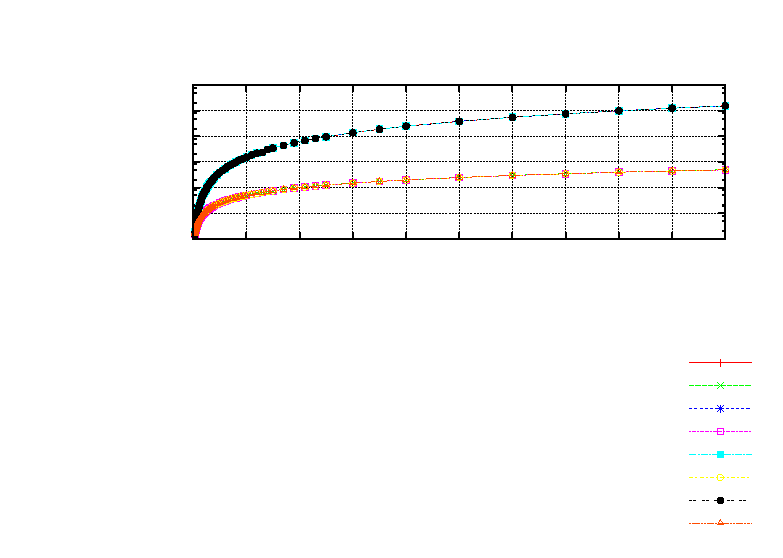
\includegraphics{ej3_frontera_star+cmf}}%
    \gplfronttext
  \end{picture}%
\endgroup
}
    \caption{Frontera para grafos Estrella+CMF}
\end{figure}

\bigskip

\par Como primer resultado, siempre es bueno ver que se cumple la cota te\'orica de complejidad.
    Siguiendo con el an\'alisis, se puede observar que mientras que las variantes quem
    menos tiempo requieren son aquellas que nos dan una soluci\'on m\'as alejada de la
    \'optima que las que requieren m\'as tiempo.

\par En particular, se puede marcar como con esta familia, se consiguien mejores resultados (no
    necesariamente \'optimos) Con las variantes de ``Mejor Vecino'' y ``Mejor Vecino con Intercambio'',
    pero a costo de tardar mucho m\'as (asint\'oticamente hablando) que aquellas opciones que
    toman como clique inicial el resultado de la heur\'istica golosa o aquellas que saltan
    al primer vecino v\'alido en lugar de recorerr toda la vecindad.

%Estrella+puente+cmf
\begin{figure}[H]
    \centering
    \fontsize{7}{10}\selectfont
    \resizebox{0.8\textwidth}{!}{% GNUPLOT: LaTeX picture with Postscript
\begingroup
  \makeatletter
  \providecommand\color[2][]{%
    \GenericError{(gnuplot) \space\space\space\@spaces}{%
      Package color not loaded in conjunction with
      terminal option `colourtext'%
    }{See the gnuplot documentation for explanation.%
    }{Either use 'blacktext' in gnuplot or load the package
      color.sty in LaTeX.}%
    \renewcommand\color[2][]{}%
  }%
  \providecommand\includegraphics[2][]{%
    \GenericError{(gnuplot) \space\space\space\@spaces}{%
      Package graphicx or graphics not loaded%
    }{See the gnuplot documentation for explanation.%
    }{The gnuplot epslatex terminal needs graphicx.sty or graphics.sty.}%
    \renewcommand\includegraphics[2][]{}%
  }%
  \providecommand\rotatebox[2]{#2}%
  \@ifundefined{ifGPcolor}{%
    \newif\ifGPcolor
    \GPcolortrue
  }{}%
  \@ifundefined{ifGPblacktext}{%
    \newif\ifGPblacktext
    \GPblacktexttrue
  }{}%
  % define a \g@addto@macro without @ in the name:
  \let\gplgaddtomacro\g@addto@macro
  % define empty templates for all commands taking text:
  \gdef\gplbacktext{}%
  \gdef\gplfronttext{}%
  \makeatother
  \ifGPblacktext
    % no textcolor at all
    \def\colorrgb#1{}%
    \def\colorgray#1{}%
  \else
    % gray or color?
    \ifGPcolor
      \def\colorrgb#1{\color[rgb]{#1}}%
      \def\colorgray#1{\color[gray]{#1}}%
      \expandafter\def\csname LTw\endcsname{\color{white}}%
      \expandafter\def\csname LTb\endcsname{\color{black}}%
      \expandafter\def\csname LTa\endcsname{\color{black}}%
      \expandafter\def\csname LT0\endcsname{\color[rgb]{1,0,0}}%
      \expandafter\def\csname LT1\endcsname{\color[rgb]{0,1,0}}%
      \expandafter\def\csname LT2\endcsname{\color[rgb]{0,0,1}}%
      \expandafter\def\csname LT3\endcsname{\color[rgb]{1,0,1}}%
      \expandafter\def\csname LT4\endcsname{\color[rgb]{0,1,1}}%
      \expandafter\def\csname LT5\endcsname{\color[rgb]{1,1,0}}%
      \expandafter\def\csname LT6\endcsname{\color[rgb]{0,0,0}}%
      \expandafter\def\csname LT7\endcsname{\color[rgb]{1,0.3,0}}%
      \expandafter\def\csname LT8\endcsname{\color[rgb]{0.5,0.5,0.5}}%
    \else
      % gray
      \def\colorrgb#1{\color{black}}%
      \def\colorgray#1{\color[gray]{#1}}%
      \expandafter\def\csname LTw\endcsname{\color{white}}%
      \expandafter\def\csname LTb\endcsname{\color{black}}%
      \expandafter\def\csname LTa\endcsname{\color{black}}%
      \expandafter\def\csname LT0\endcsname{\color{black}}%
      \expandafter\def\csname LT1\endcsname{\color{black}}%
      \expandafter\def\csname LT2\endcsname{\color{black}}%
      \expandafter\def\csname LT3\endcsname{\color{black}}%
      \expandafter\def\csname LT4\endcsname{\color{black}}%
      \expandafter\def\csname LT5\endcsname{\color{black}}%
      \expandafter\def\csname LT6\endcsname{\color{black}}%
      \expandafter\def\csname LT7\endcsname{\color{black}}%
      \expandafter\def\csname LT8\endcsname{\color{black}}%
    \fi
  \fi
  \setlength{\unitlength}{0.0500bp}%
  \begin{picture}(7200.00,5040.00)%
    \gplgaddtomacro\gplbacktext{%
      \csname LTb\endcsname%
      \put(1034,1375){\makebox(0,0)[r]{\strut{} 10}}%
      \csname LTb\endcsname%
      \put(1034,1875){\makebox(0,0)[r]{\strut{} 20}}%
      \csname LTb\endcsname%
      \put(1034,2376){\makebox(0,0)[r]{\strut{} 30}}%
      \csname LTb\endcsname%
      \put(1034,2877){\makebox(0,0)[r]{\strut{} 40}}%
      \csname LTb\endcsname%
      \put(1034,3378){\makebox(0,0)[r]{\strut{} 50}}%
      \csname LTb\endcsname%
      \put(1034,3878){\makebox(0,0)[r]{\strut{} 60}}%
      \csname LTb\endcsname%
      \put(1034,4379){\makebox(0,0)[r]{\strut{} 70}}%
      \csname LTb\endcsname%
      \put(1165,704){\makebox(0,0){\strut{} 0}}%
      \csname LTb\endcsname%
      \put(1729,704){\makebox(0,0){\strut{} 500}}%
      \csname LTb\endcsname%
      \put(2292,704){\makebox(0,0){\strut{} 1000}}%
      \csname LTb\endcsname%
      \put(2856,704){\makebox(0,0){\strut{} 1500}}%
      \csname LTb\endcsname%
      \put(3420,704){\makebox(0,0){\strut{} 2000}}%
      \csname LTb\endcsname%
      \put(3984,704){\makebox(0,0){\strut{} 2500}}%
      \csname LTb\endcsname%
      \put(4548,704){\makebox(0,0){\strut{} 3000}}%
      \csname LTb\endcsname%
      \put(5112,704){\makebox(0,0){\strut{} 3500}}%
      \csname LTb\endcsname%
      \put(5675,704){\makebox(0,0){\strut{} 4000}}%
      \csname LTb\endcsname%
      \put(6239,704){\makebox(0,0){\strut{} 4500}}%
      \csname LTb\endcsname%
      \put(6803,704){\makebox(0,0){\strut{} 5000}}%
      \put(176,2651){\rotatebox{-270}{\makebox(0,0){\strut{}Tiempo ($microsegundos^{\sfrac{1}{5}}$)}}}%
      \put(396,2651){\rotatebox{-270}{\makebox(0,0){\strut{}(Escala Lineal)}}}%
      \put(3984,374){\makebox(0,0){\strut{}Cantidad de Nodos}}%
      \put(3984,154){\makebox(0,0){\strut{}(Escala Lineal)}}%
      \put(3984,4709){\makebox(0,0){\strut{}Tiempo de ejecución conforme aumenta la cantidad de nodos}}%
    }%
    \gplgaddtomacro\gplfronttext{%
      \csname LTb\endcsname%
      \put(3928,4269){\makebox(0,0)[r]{\strut{}Primer Vecino}}%
      \csname LTb\endcsname%
      \put(3928,4049){\makebox(0,0)[r]{\strut{}Primer Vecino con golosa}}%
      \csname LTb\endcsname%
      \put(3928,3829){\makebox(0,0)[r]{\strut{}Primer Vecino con intercambio}}%
      \csname LTb\endcsname%
      \put(3928,3609){\makebox(0,0)[r]{\strut{}Primer Vecino con intercambio y golosa}}%
      \csname LTb\endcsname%
      \put(3928,3389){\makebox(0,0)[r]{\strut{}Mejor Vecino}}%
      \csname LTb\endcsname%
      \put(3928,3169){\makebox(0,0)[r]{\strut{}Mejor Vecino con golosa}}%
      \csname LTb\endcsname%
      \put(3928,2949){\makebox(0,0)[r]{\strut{}Mejor Vecino con intercambio}}%
      \csname LTb\endcsname%
      \put(3928,2729){\makebox(0,0)[r]{\strut{}Mejor Vecino con intercambio y golosa}}%
      \csname LTb\endcsname%
      \put(3928,2509){\makebox(0,0)[r]{\strut{}Cota teórica superior $\mathcal O(n)$}}%
    }%
    \gplbacktext
    \put(0,0){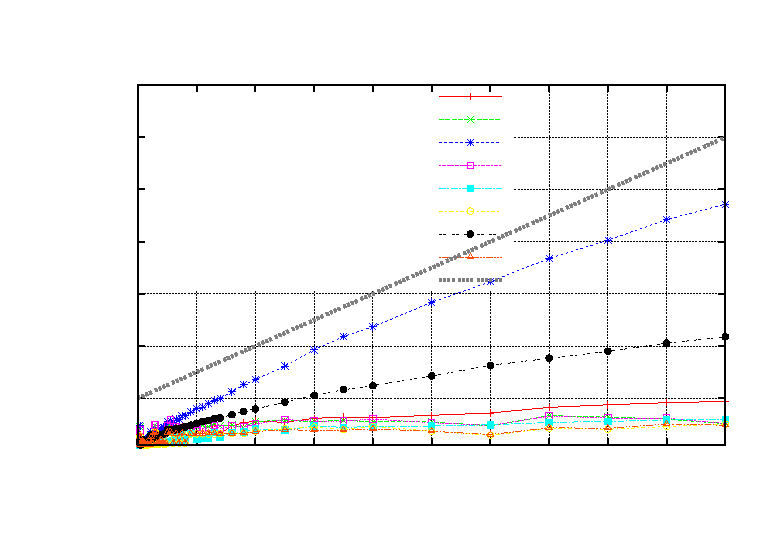
\includegraphics{ej3_nodos_star+bridge+cmf}}%
    \gplfronttext
  \end{picture}%
\endgroup
}
    \caption{Complejidad temporal para grafos Estrella+Puente+CMF}
\end{figure}

\begin{figure}[H]
    \centering
    \fontsize{7}{10}\selectfont
    \resizebox{0.8\textwidth}{!}{% GNUPLOT: LaTeX picture with Postscript
\begingroup
  \makeatletter
  \providecommand\color[2][]{%
    \GenericError{(gnuplot) \space\space\space\@spaces}{%
      Package color not loaded in conjunction with
      terminal option `colourtext'%
    }{See the gnuplot documentation for explanation.%
    }{Either use 'blacktext' in gnuplot or load the package
      color.sty in LaTeX.}%
    \renewcommand\color[2][]{}%
  }%
  \providecommand\includegraphics[2][]{%
    \GenericError{(gnuplot) \space\space\space\@spaces}{%
      Package graphicx or graphics not loaded%
    }{See the gnuplot documentation for explanation.%
    }{The gnuplot epslatex terminal needs graphicx.sty or graphics.sty.}%
    \renewcommand\includegraphics[2][]{}%
  }%
  \providecommand\rotatebox[2]{#2}%
  \@ifundefined{ifGPcolor}{%
    \newif\ifGPcolor
    \GPcolortrue
  }{}%
  \@ifundefined{ifGPblacktext}{%
    \newif\ifGPblacktext
    \GPblacktexttrue
  }{}%
  % define a \g@addto@macro without @ in the name:
  \let\gplgaddtomacro\g@addto@macro
  % define empty templates for all commands taking text:
  \gdef\gplbacktext{}%
  \gdef\gplfronttext{}%
  \makeatother
  \ifGPblacktext
    % no textcolor at all
    \def\colorrgb#1{}%
    \def\colorgray#1{}%
  \else
    % gray or color?
    \ifGPcolor
      \def\colorrgb#1{\color[rgb]{#1}}%
      \def\colorgray#1{\color[gray]{#1}}%
      \expandafter\def\csname LTw\endcsname{\color{white}}%
      \expandafter\def\csname LTb\endcsname{\color{black}}%
      \expandafter\def\csname LTa\endcsname{\color{black}}%
      \expandafter\def\csname LT0\endcsname{\color[rgb]{1,0,0}}%
      \expandafter\def\csname LT1\endcsname{\color[rgb]{0,1,0}}%
      \expandafter\def\csname LT2\endcsname{\color[rgb]{0,0,1}}%
      \expandafter\def\csname LT3\endcsname{\color[rgb]{1,0,1}}%
      \expandafter\def\csname LT4\endcsname{\color[rgb]{0,1,1}}%
      \expandafter\def\csname LT5\endcsname{\color[rgb]{1,1,0}}%
      \expandafter\def\csname LT6\endcsname{\color[rgb]{0,0,0}}%
      \expandafter\def\csname LT7\endcsname{\color[rgb]{1,0.3,0}}%
      \expandafter\def\csname LT8\endcsname{\color[rgb]{0.5,0.5,0.5}}%
    \else
      % gray
      \def\colorrgb#1{\color{black}}%
      \def\colorgray#1{\color[gray]{#1}}%
      \expandafter\def\csname LTw\endcsname{\color{white}}%
      \expandafter\def\csname LTb\endcsname{\color{black}}%
      \expandafter\def\csname LTa\endcsname{\color{black}}%
      \expandafter\def\csname LT0\endcsname{\color{black}}%
      \expandafter\def\csname LT1\endcsname{\color{black}}%
      \expandafter\def\csname LT2\endcsname{\color{black}}%
      \expandafter\def\csname LT3\endcsname{\color{black}}%
      \expandafter\def\csname LT4\endcsname{\color{black}}%
      \expandafter\def\csname LT5\endcsname{\color{black}}%
      \expandafter\def\csname LT6\endcsname{\color{black}}%
      \expandafter\def\csname LT7\endcsname{\color{black}}%
      \expandafter\def\csname LT8\endcsname{\color{black}}%
    \fi
  \fi
  \setlength{\unitlength}{0.0500bp}%
  \begin{picture}(7200.00,5040.00)%
    \gplgaddtomacro\gplbacktext{%
      \csname LTb\endcsname%
      \put(1562,2904){\makebox(0,0)[r]{\strut{} 1}}%
      \csname LTb\endcsname%
      \put(1562,3115){\makebox(0,0)[r]{\strut{} 10}}%
      \csname LTb\endcsname%
      \put(1562,3325){\makebox(0,0)[r]{\strut{} 100}}%
      \csname LTb\endcsname%
      \put(1562,3536){\makebox(0,0)[r]{\strut{} 1000}}%
      \csname LTb\endcsname%
      \put(1562,3747){\makebox(0,0)[r]{\strut{} 10000}}%
      \csname LTb\endcsname%
      \put(1562,3958){\makebox(0,0)[r]{\strut{} 100000}}%
      \csname LTb\endcsname%
      \put(1562,4168){\makebox(0,0)[r]{\strut{} 1e+06}}%
      \csname LTb\endcsname%
      \put(1562,4379){\makebox(0,0)[r]{\strut{} 1e+07}}%
      \csname LTb\endcsname%
      \put(1694,2684){\makebox(0,0){\strut{} 0}}%
      \csname LTb\endcsname%
      \put(2205,2684){\makebox(0,0){\strut{} 500}}%
      \csname LTb\endcsname%
      \put(2716,2684){\makebox(0,0){\strut{} 1000}}%
      \csname LTb\endcsname%
      \put(3227,2684){\makebox(0,0){\strut{} 1500}}%
      \csname LTb\endcsname%
      \put(3738,2684){\makebox(0,0){\strut{} 2000}}%
      \csname LTb\endcsname%
      \put(4249,2684){\makebox(0,0){\strut{} 2500}}%
      \csname LTb\endcsname%
      \put(4759,2684){\makebox(0,0){\strut{} 3000}}%
      \csname LTb\endcsname%
      \put(5270,2684){\makebox(0,0){\strut{} 3500}}%
      \csname LTb\endcsname%
      \put(5781,2684){\makebox(0,0){\strut{} 4000}}%
      \csname LTb\endcsname%
      \put(6292,2684){\makebox(0,0){\strut{} 4500}}%
      \csname LTb\endcsname%
      \put(6803,2684){\makebox(0,0){\strut{} 5000}}%
      \put(176,3641){\rotatebox{-270}{\makebox(0,0){\strut{}Frontera}}}%
      \put(396,3641){\rotatebox{-270}{\makebox(0,0){\strut{}(Escala Logaritmica)}}}%
      \put(4248,2354){\makebox(0,0){\strut{}Cantidad de Nodos}}%
      \put(4248,2134){\makebox(0,0){\strut{}(Escala Lineal)}}%
      \put(4248,4709){\makebox(0,0){\strut{}Relacion Frontera/Nodos}}%
    }%
    \gplgaddtomacro\gplfronttext{%
      \csname LTb\endcsname%
      \put(6329,1713){\makebox(0,0)[r]{\strut{}Primer Vecino}}%
      \csname LTb\endcsname%
      \put(6329,1493){\makebox(0,0)[r]{\strut{}Primer Vecino con golosa}}%
      \csname LTb\endcsname%
      \put(6329,1273){\makebox(0,0)[r]{\strut{}Primer Vecino con intercambio}}%
      \csname LTb\endcsname%
      \put(6329,1053){\makebox(0,0)[r]{\strut{}Primer Vecino con intercambio y golosa}}%
      \csname LTb\endcsname%
      \put(6329,833){\makebox(0,0)[r]{\strut{}Mejor Vecino}}%
      \csname LTb\endcsname%
      \put(6329,613){\makebox(0,0)[r]{\strut{}Mejor Vecino con golosa}}%
      \csname LTb\endcsname%
      \put(6329,393){\makebox(0,0)[r]{\strut{}Mejor Vecino con intercambio}}%
      \csname LTb\endcsname%
      \put(6329,173){\makebox(0,0)[r]{\strut{}Mejor Vecino con intercambio y golosa}}%
    }%
    \gplbacktext
    \put(0,0){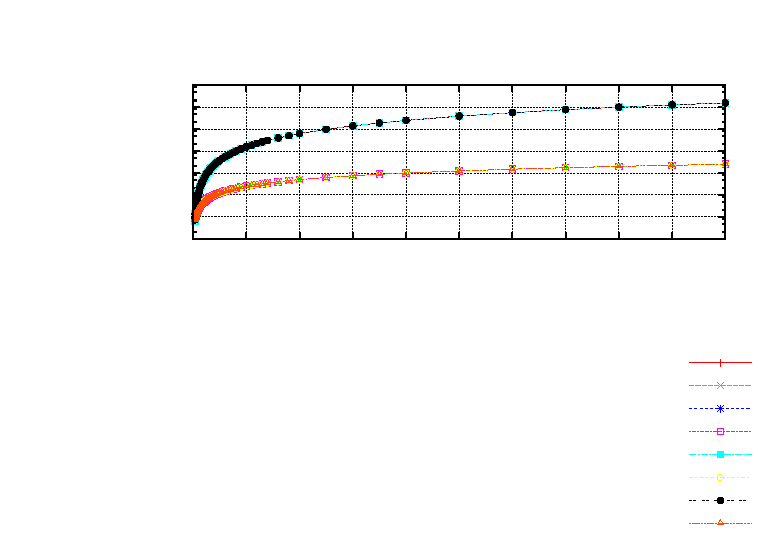
\includegraphics{ej3_frontera_star+bridge+cmf}}%
    \gplfronttext
  \end{picture}%
\endgroup
}
    \caption{Frontera grafos Estrella+Puente+CMF}
\end{figure}

\bigskip

\par Id\'entico a la familia anterior, se ve exactamente el mismo comportamiento
    aqu\'i que en la familia $Estrella+CMF$.

%Arboles
\begin{figure}[H]
    \centering
    \fontsize{7}{10}\selectfont
    \resizebox{0.8\textwidth}{!}{% GNUPLOT: LaTeX picture with Postscript
\begingroup
  \makeatletter
  \providecommand\color[2][]{%
    \GenericError{(gnuplot) \space\space\space\@spaces}{%
      Package color not loaded in conjunction with
      terminal option `colourtext'%
    }{See the gnuplot documentation for explanation.%
    }{Either use 'blacktext' in gnuplot or load the package
      color.sty in LaTeX.}%
    \renewcommand\color[2][]{}%
  }%
  \providecommand\includegraphics[2][]{%
    \GenericError{(gnuplot) \space\space\space\@spaces}{%
      Package graphicx or graphics not loaded%
    }{See the gnuplot documentation for explanation.%
    }{The gnuplot epslatex terminal needs graphicx.sty or graphics.sty.}%
    \renewcommand\includegraphics[2][]{}%
  }%
  \providecommand\rotatebox[2]{#2}%
  \@ifundefined{ifGPcolor}{%
    \newif\ifGPcolor
    \GPcolortrue
  }{}%
  \@ifundefined{ifGPblacktext}{%
    \newif\ifGPblacktext
    \GPblacktexttrue
  }{}%
  % define a \g@addto@macro without @ in the name:
  \let\gplgaddtomacro\g@addto@macro
  % define empty templates for all commands taking text:
  \gdef\gplbacktext{}%
  \gdef\gplfronttext{}%
  \makeatother
  \ifGPblacktext
    % no textcolor at all
    \def\colorrgb#1{}%
    \def\colorgray#1{}%
  \else
    % gray or color?
    \ifGPcolor
      \def\colorrgb#1{\color[rgb]{#1}}%
      \def\colorgray#1{\color[gray]{#1}}%
      \expandafter\def\csname LTw\endcsname{\color{white}}%
      \expandafter\def\csname LTb\endcsname{\color{black}}%
      \expandafter\def\csname LTa\endcsname{\color{black}}%
      \expandafter\def\csname LT0\endcsname{\color[rgb]{1,0,0}}%
      \expandafter\def\csname LT1\endcsname{\color[rgb]{0,1,0}}%
      \expandafter\def\csname LT2\endcsname{\color[rgb]{0,0,1}}%
      \expandafter\def\csname LT3\endcsname{\color[rgb]{1,0,1}}%
      \expandafter\def\csname LT4\endcsname{\color[rgb]{0,1,1}}%
      \expandafter\def\csname LT5\endcsname{\color[rgb]{1,1,0}}%
      \expandafter\def\csname LT6\endcsname{\color[rgb]{0,0,0}}%
      \expandafter\def\csname LT7\endcsname{\color[rgb]{1,0.3,0}}%
      \expandafter\def\csname LT8\endcsname{\color[rgb]{0.5,0.5,0.5}}%
    \else
      % gray
      \def\colorrgb#1{\color{black}}%
      \def\colorgray#1{\color[gray]{#1}}%
      \expandafter\def\csname LTw\endcsname{\color{white}}%
      \expandafter\def\csname LTb\endcsname{\color{black}}%
      \expandafter\def\csname LTa\endcsname{\color{black}}%
      \expandafter\def\csname LT0\endcsname{\color{black}}%
      \expandafter\def\csname LT1\endcsname{\color{black}}%
      \expandafter\def\csname LT2\endcsname{\color{black}}%
      \expandafter\def\csname LT3\endcsname{\color{black}}%
      \expandafter\def\csname LT4\endcsname{\color{black}}%
      \expandafter\def\csname LT5\endcsname{\color{black}}%
      \expandafter\def\csname LT6\endcsname{\color{black}}%
      \expandafter\def\csname LT7\endcsname{\color{black}}%
      \expandafter\def\csname LT8\endcsname{\color{black}}%
    \fi
  \fi
  \setlength{\unitlength}{0.0500bp}%
  \begin{picture}(7200.00,5040.00)%
    \gplgaddtomacro\gplbacktext{%
      \csname LTb\endcsname%
      \put(1034,1318){\makebox(0,0)[r]{\strut{} 10}}%
      \csname LTb\endcsname%
      \put(1034,1755){\makebox(0,0)[r]{\strut{} 20}}%
      \csname LTb\endcsname%
      \put(1034,2192){\makebox(0,0)[r]{\strut{} 30}}%
      \csname LTb\endcsname%
      \put(1034,2630){\makebox(0,0)[r]{\strut{} 40}}%
      \csname LTb\endcsname%
      \put(1034,3067){\makebox(0,0)[r]{\strut{} 50}}%
      \csname LTb\endcsname%
      \put(1034,3504){\makebox(0,0)[r]{\strut{} 60}}%
      \csname LTb\endcsname%
      \put(1034,3942){\makebox(0,0)[r]{\strut{} 70}}%
      \csname LTb\endcsname%
      \put(1034,4379){\makebox(0,0)[r]{\strut{} 80}}%
      \csname LTb\endcsname%
      \put(1165,704){\makebox(0,0){\strut{} 0}}%
      \csname LTb\endcsname%
      \put(1729,704){\makebox(0,0){\strut{} 500}}%
      \csname LTb\endcsname%
      \put(2292,704){\makebox(0,0){\strut{} 1000}}%
      \csname LTb\endcsname%
      \put(2856,704){\makebox(0,0){\strut{} 1500}}%
      \csname LTb\endcsname%
      \put(3420,704){\makebox(0,0){\strut{} 2000}}%
      \csname LTb\endcsname%
      \put(3984,704){\makebox(0,0){\strut{} 2500}}%
      \csname LTb\endcsname%
      \put(4548,704){\makebox(0,0){\strut{} 3000}}%
      \csname LTb\endcsname%
      \put(5112,704){\makebox(0,0){\strut{} 3500}}%
      \csname LTb\endcsname%
      \put(5675,704){\makebox(0,0){\strut{} 4000}}%
      \csname LTb\endcsname%
      \put(6239,704){\makebox(0,0){\strut{} 4500}}%
      \csname LTb\endcsname%
      \put(6803,704){\makebox(0,0){\strut{} 5000}}%
      \put(176,2651){\rotatebox{-270}{\makebox(0,0){\strut{}Tiempo ($nanosegundos^{\sfrac{1}{5}}$)}}}%
      \put(396,2651){\rotatebox{-270}{\makebox(0,0){\strut{}(Escala Lineal)}}}%
      \put(3984,374){\makebox(0,0){\strut{}Cantidad de Nodos}}%
      \put(3984,154){\makebox(0,0){\strut{}(Escala Lineal)}}%
      \put(3984,4709){\makebox(0,0){\strut{}Tiempo de ejecución conforme aumenta la cantidad de nodos}}%
    }%
    \gplgaddtomacro\gplfronttext{%
      \csname LTb\endcsname%
      \put(3975,4269){\makebox(0,0)[r]{\strut{}Primer Vecino}}%
      \csname LTb\endcsname%
      \put(3975,4049){\makebox(0,0)[r]{\strut{}Primer Vecino con golosa}}%
      \csname LTb\endcsname%
      \put(3975,3829){\makebox(0,0)[r]{\strut{}Primer Vecino con intercambio}}%
      \csname LTb\endcsname%
      \put(3975,3609){\makebox(0,0)[r]{\strut{}Primer Vecino con intercambio y golosa}}%
      \csname LTb\endcsname%
      \put(3975,3389){\makebox(0,0)[r]{\strut{}Mejor Vecino}}%
      \csname LTb\endcsname%
      \put(3975,3169){\makebox(0,0)[r]{\strut{}Mejor Vecino con golosa}}%
      \csname LTb\endcsname%
      \put(3975,2949){\makebox(0,0)[r]{\strut{}Mejor Vecino con intercambio}}%
      \csname LTb\endcsname%
      \put(3975,2729){\makebox(0,0)[r]{\strut{}Mejor Vecino con intercambio y golosa}}%
      \csname LTb\endcsname%
      \put(3975,2509){\makebox(0,0)[r]{\strut{}Cota teórica superior $\mathcal O(n)$}}%
    }%
    \gplbacktext
    \put(0,0){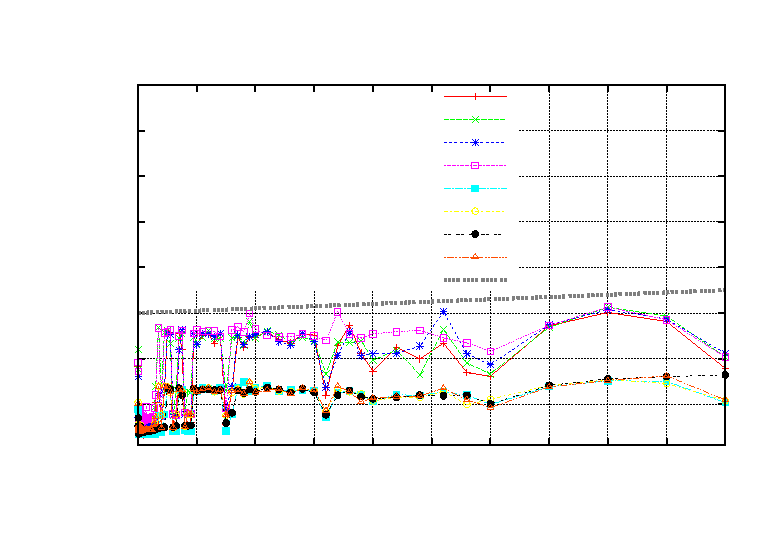
\includegraphics{ej3_nodos_tree}}%
    \gplfronttext
  \end{picture}%
\endgroup
}
    \caption{Complejidad temporal para \'Arboles}
\end{figure}

\begin{figure}[H]
    \centering
    \fontsize{7}{10}\selectfont
    \resizebox{0.8\textwidth}{!}{% GNUPLOT: LaTeX picture with Postscript
\begingroup
  \makeatletter
  \providecommand\color[2][]{%
    \GenericError{(gnuplot) \space\space\space\@spaces}{%
      Package color not loaded in conjunction with
      terminal option `colourtext'%
    }{See the gnuplot documentation for explanation.%
    }{Either use 'blacktext' in gnuplot or load the package
      color.sty in LaTeX.}%
    \renewcommand\color[2][]{}%
  }%
  \providecommand\includegraphics[2][]{%
    \GenericError{(gnuplot) \space\space\space\@spaces}{%
      Package graphicx or graphics not loaded%
    }{See the gnuplot documentation for explanation.%
    }{The gnuplot epslatex terminal needs graphicx.sty or graphics.sty.}%
    \renewcommand\includegraphics[2][]{}%
  }%
  \providecommand\rotatebox[2]{#2}%
  \@ifundefined{ifGPcolor}{%
    \newif\ifGPcolor
    \GPcolortrue
  }{}%
  \@ifundefined{ifGPblacktext}{%
    \newif\ifGPblacktext
    \GPblacktexttrue
  }{}%
  % define a \g@addto@macro without @ in the name:
  \let\gplgaddtomacro\g@addto@macro
  % define empty templates for all commands taking text:
  \gdef\gplbacktext{}%
  \gdef\gplfronttext{}%
  \makeatother
  \ifGPblacktext
    % no textcolor at all
    \def\colorrgb#1{}%
    \def\colorgray#1{}%
  \else
    % gray or color?
    \ifGPcolor
      \def\colorrgb#1{\color[rgb]{#1}}%
      \def\colorgray#1{\color[gray]{#1}}%
      \expandafter\def\csname LTw\endcsname{\color{white}}%
      \expandafter\def\csname LTb\endcsname{\color{black}}%
      \expandafter\def\csname LTa\endcsname{\color{black}}%
      \expandafter\def\csname LT0\endcsname{\color[rgb]{1,0,0}}%
      \expandafter\def\csname LT1\endcsname{\color[rgb]{0,1,0}}%
      \expandafter\def\csname LT2\endcsname{\color[rgb]{0,0,1}}%
      \expandafter\def\csname LT3\endcsname{\color[rgb]{1,0,1}}%
      \expandafter\def\csname LT4\endcsname{\color[rgb]{0,1,1}}%
      \expandafter\def\csname LT5\endcsname{\color[rgb]{1,1,0}}%
      \expandafter\def\csname LT6\endcsname{\color[rgb]{0,0,0}}%
      \expandafter\def\csname LT7\endcsname{\color[rgb]{1,0.3,0}}%
      \expandafter\def\csname LT8\endcsname{\color[rgb]{0.5,0.5,0.5}}%
    \else
      % gray
      \def\colorrgb#1{\color{black}}%
      \def\colorgray#1{\color[gray]{#1}}%
      \expandafter\def\csname LTw\endcsname{\color{white}}%
      \expandafter\def\csname LTb\endcsname{\color{black}}%
      \expandafter\def\csname LTa\endcsname{\color{black}}%
      \expandafter\def\csname LT0\endcsname{\color{black}}%
      \expandafter\def\csname LT1\endcsname{\color{black}}%
      \expandafter\def\csname LT2\endcsname{\color{black}}%
      \expandafter\def\csname LT3\endcsname{\color{black}}%
      \expandafter\def\csname LT4\endcsname{\color{black}}%
      \expandafter\def\csname LT5\endcsname{\color{black}}%
      \expandafter\def\csname LT6\endcsname{\color{black}}%
      \expandafter\def\csname LT7\endcsname{\color{black}}%
      \expandafter\def\csname LT8\endcsname{\color{black}}%
    \fi
  \fi
  \setlength{\unitlength}{0.0500bp}%
  \begin{picture}(7200.00,5040.00)%
    \gplgaddtomacro\gplbacktext{%
      \csname LTb\endcsname%
      \put(1034,2904){\makebox(0,0)[r]{\strut{} 2}}%
      \csname LTb\endcsname%
      \put(1034,3052){\makebox(0,0)[r]{\strut{} 4}}%
      \csname LTb\endcsname%
      \put(1034,3199){\makebox(0,0)[r]{\strut{} 6}}%
      \csname LTb\endcsname%
      \put(1034,3347){\makebox(0,0)[r]{\strut{} 8}}%
      \csname LTb\endcsname%
      \put(1034,3494){\makebox(0,0)[r]{\strut{} 10}}%
      \csname LTb\endcsname%
      \put(1034,3642){\makebox(0,0)[r]{\strut{} 12}}%
      \csname LTb\endcsname%
      \put(1034,3789){\makebox(0,0)[r]{\strut{} 14}}%
      \csname LTb\endcsname%
      \put(1034,3937){\makebox(0,0)[r]{\strut{} 16}}%
      \csname LTb\endcsname%
      \put(1034,4084){\makebox(0,0)[r]{\strut{} 18}}%
      \csname LTb\endcsname%
      \put(1034,4232){\makebox(0,0)[r]{\strut{} 20}}%
      \csname LTb\endcsname%
      \put(1034,4379){\makebox(0,0)[r]{\strut{} 22}}%
      \put(176,3641){\rotatebox{-270}{\makebox(0,0){\strut{}Frontera}}}%
      \put(396,3641){\rotatebox{-270}{\makebox(0,0){\strut{}(Escala Lineal)}}}%
      \put(3984,2354){\makebox(0,0){\strut{}Cantidad de Nodos}}%
      \put(3984,2134){\makebox(0,0){\strut{}(Escala Lineal)}}%
      \put(3984,4709){\makebox(0,0){\strut{}Relacion Frontera/Nodos}}%
    }%
    \gplgaddtomacro\gplfronttext{%
      \csname LTb\endcsname%
      \put(6065,1713){\makebox(0,0)[r]{\strut{}Primer Vecino}}%
      \csname LTb\endcsname%
      \put(6065,1493){\makebox(0,0)[r]{\strut{}Primer Vecino con golosa}}%
      \csname LTb\endcsname%
      \put(6065,1273){\makebox(0,0)[r]{\strut{}Primer Vecino con intercambio}}%
      \csname LTb\endcsname%
      \put(6065,1053){\makebox(0,0)[r]{\strut{}Primer Vecino con intercambio y golosa}}%
      \csname LTb\endcsname%
      \put(6065,833){\makebox(0,0)[r]{\strut{}Mejor Vecino}}%
      \csname LTb\endcsname%
      \put(6065,613){\makebox(0,0)[r]{\strut{}Mejor Vecino con golosa}}%
      \csname LTb\endcsname%
      \put(6065,393){\makebox(0,0)[r]{\strut{}Mejor Vecino con intercambio}}%
      \csname LTb\endcsname%
      \put(6065,173){\makebox(0,0)[r]{\strut{}Mejor Vecino con intercambio y golosa}}%
    }%
    \gplbacktext
    \put(0,0){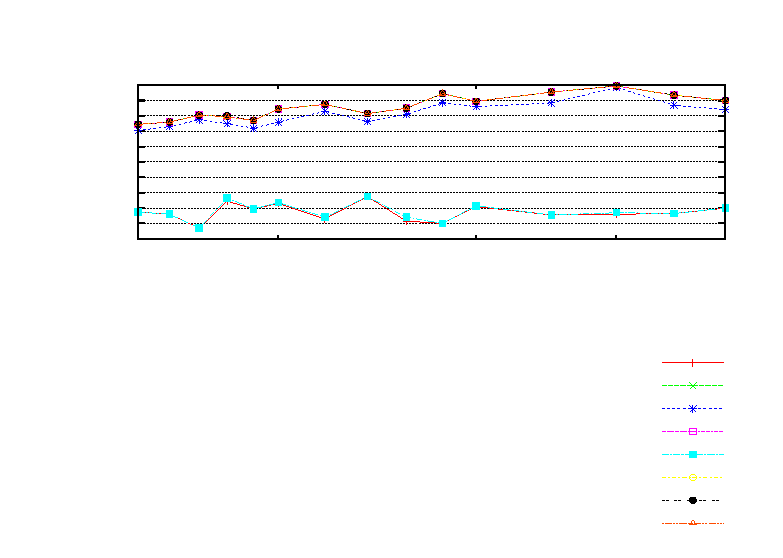
\includegraphics{ej3_frontera_tree}}%
    \gplfronttext
  \end{picture}%
\endgroup
}
    \caption{Frontera para \'Arboles}
\end{figure}

\bigskip

\par Para esta famili nos encontramos finalmente con un resultado un tanto err\'atico.
    Nuevamente, se cumple con la complejidad calculada, pero ahora se nota
    una gran variacion a medida que crecen de tama\~no las instancias de entrada.

\par Como se ha visto, los \'arboles es una familia que contiene a muchas instancias de
    las familias $Estrella+CMF$ y $Estrella+Puente+CMF$ (en particular, cuando la $CMF$
    es de tama\~no dos). Por lo tanto, es l\'ogico esperar un comportamiento m\'as
    oscilante y a su vez no obtener necesariamente una buena soluci\'on aproximada.

\par Cabe destacar, que para esta familia, se invierte lo que ven\'iamos observando en
    las familias anteriores (a pesar de estas tener una intersecci\'on no vac\'ia con
    la familia de \'arboles). Aqu\'i, las f\'amilias que m\'as r\'apido terminan son
    las que realizan los mejores saltos dentro de la vecindad. Y a su vez, podemos
    observar que para la variante de ``Mejor Vecino con Intercambio'', se
    obtienen los mejores resultados. Es decir, es una variante que requiere poco
    tiempo y da mejores resultados que los dem\'as para esta familia.

%Ruedas
\begin{figure}[H]
    \centering
    \fontsize{7}{10}\selectfont
    \resizebox{0.8\textwidth}{!}{% GNUPLOT: LaTeX picture with Postscript
\begingroup
  \makeatletter
  \providecommand\color[2][]{%
    \GenericError{(gnuplot) \space\space\space\@spaces}{%
      Package color not loaded in conjunction with
      terminal option `colourtext'%
    }{See the gnuplot documentation for explanation.%
    }{Either use 'blacktext' in gnuplot or load the package
      color.sty in LaTeX.}%
    \renewcommand\color[2][]{}%
  }%
  \providecommand\includegraphics[2][]{%
    \GenericError{(gnuplot) \space\space\space\@spaces}{%
      Package graphicx or graphics not loaded%
    }{See the gnuplot documentation for explanation.%
    }{The gnuplot epslatex terminal needs graphicx.sty or graphics.sty.}%
    \renewcommand\includegraphics[2][]{}%
  }%
  \providecommand\rotatebox[2]{#2}%
  \@ifundefined{ifGPcolor}{%
    \newif\ifGPcolor
    \GPcolortrue
  }{}%
  \@ifundefined{ifGPblacktext}{%
    \newif\ifGPblacktext
    \GPblacktexttrue
  }{}%
  % define a \g@addto@macro without @ in the name:
  \let\gplgaddtomacro\g@addto@macro
  % define empty templates for all commands taking text:
  \gdef\gplbacktext{}%
  \gdef\gplfronttext{}%
  \makeatother
  \ifGPblacktext
    % no textcolor at all
    \def\colorrgb#1{}%
    \def\colorgray#1{}%
  \else
    % gray or color?
    \ifGPcolor
      \def\colorrgb#1{\color[rgb]{#1}}%
      \def\colorgray#1{\color[gray]{#1}}%
      \expandafter\def\csname LTw\endcsname{\color{white}}%
      \expandafter\def\csname LTb\endcsname{\color{black}}%
      \expandafter\def\csname LTa\endcsname{\color{black}}%
      \expandafter\def\csname LT0\endcsname{\color[rgb]{1,0,0}}%
      \expandafter\def\csname LT1\endcsname{\color[rgb]{0,1,0}}%
      \expandafter\def\csname LT2\endcsname{\color[rgb]{0,0,1}}%
      \expandafter\def\csname LT3\endcsname{\color[rgb]{1,0,1}}%
      \expandafter\def\csname LT4\endcsname{\color[rgb]{0,1,1}}%
      \expandafter\def\csname LT5\endcsname{\color[rgb]{1,1,0}}%
      \expandafter\def\csname LT6\endcsname{\color[rgb]{0,0,0}}%
      \expandafter\def\csname LT7\endcsname{\color[rgb]{1,0.3,0}}%
      \expandafter\def\csname LT8\endcsname{\color[rgb]{0.5,0.5,0.5}}%
    \else
      % gray
      \def\colorrgb#1{\color{black}}%
      \def\colorgray#1{\color[gray]{#1}}%
      \expandafter\def\csname LTw\endcsname{\color{white}}%
      \expandafter\def\csname LTb\endcsname{\color{black}}%
      \expandafter\def\csname LTa\endcsname{\color{black}}%
      \expandafter\def\csname LT0\endcsname{\color{black}}%
      \expandafter\def\csname LT1\endcsname{\color{black}}%
      \expandafter\def\csname LT2\endcsname{\color{black}}%
      \expandafter\def\csname LT3\endcsname{\color{black}}%
      \expandafter\def\csname LT4\endcsname{\color{black}}%
      \expandafter\def\csname LT5\endcsname{\color{black}}%
      \expandafter\def\csname LT6\endcsname{\color{black}}%
      \expandafter\def\csname LT7\endcsname{\color{black}}%
      \expandafter\def\csname LT8\endcsname{\color{black}}%
    \fi
  \fi
  \setlength{\unitlength}{0.0500bp}%
  \begin{picture}(7200.00,5040.00)%
    \gplgaddtomacro\gplbacktext{%
      \csname LTb\endcsname%
      \put(1034,3124){\makebox(0,0)[r]{\strut{} 0}}%
      \csname LTb\endcsname%
      \put(1034,3333){\makebox(0,0)[r]{\strut{} 10}}%
      \csname LTb\endcsname%
      \put(1034,3542){\makebox(0,0)[r]{\strut{} 20}}%
      \csname LTb\endcsname%
      \put(1034,3752){\makebox(0,0)[r]{\strut{} 30}}%
      \csname LTb\endcsname%
      \put(1034,3961){\makebox(0,0)[r]{\strut{} 40}}%
      \csname LTb\endcsname%
      \put(1034,4170){\makebox(0,0)[r]{\strut{} 50}}%
      \csname LTb\endcsname%
      \put(1034,4379){\makebox(0,0)[r]{\strut{} 60}}%
      \csname LTb\endcsname%
      \put(1166,2904){\makebox(0,0){\strut{} 0}}%
      \csname LTb\endcsname%
      \put(1730,2904){\makebox(0,0){\strut{} 1000}}%
      \csname LTb\endcsname%
      \put(2293,2904){\makebox(0,0){\strut{} 2000}}%
      \csname LTb\endcsname%
      \put(2857,2904){\makebox(0,0){\strut{} 3000}}%
      \csname LTb\endcsname%
      \put(3421,2904){\makebox(0,0){\strut{} 4000}}%
      \csname LTb\endcsname%
      \put(3985,2904){\makebox(0,0){\strut{} 5000}}%
      \csname LTb\endcsname%
      \put(4548,2904){\makebox(0,0){\strut{} 6000}}%
      \csname LTb\endcsname%
      \put(5112,2904){\makebox(0,0){\strut{} 7000}}%
      \csname LTb\endcsname%
      \put(5676,2904){\makebox(0,0){\strut{} 8000}}%
      \csname LTb\endcsname%
      \put(6239,2904){\makebox(0,0){\strut{} 9000}}%
      \csname LTb\endcsname%
      \put(6803,2904){\makebox(0,0){\strut{} 10000}}%
      \put(176,3751){\rotatebox{-270}{\makebox(0,0){\strut{}Tiempo ($nanosegundos^{\sfrac{1}{5}}$)}}}%
      \put(396,3751){\rotatebox{-270}{\makebox(0,0){\strut{}(Escala Lineal)}}}%
      \put(3984,2574){\makebox(0,0){\strut{}Cantidad de Nodos}}%
      \put(3984,2354){\makebox(0,0){\strut{}(Escala Lineal)}}%
      \put(3984,4709){\makebox(0,0){\strut{}Tiempo de ejecución conforme aumenta la cantidad de nodos}}%
    }%
    \gplgaddtomacro\gplfronttext{%
      \csname LTb\endcsname%
      \put(6065,1933){\makebox(0,0)[r]{\strut{}Primer Vecino}}%
      \csname LTb\endcsname%
      \put(6065,1713){\makebox(0,0)[r]{\strut{}Primer Vecino con golosa}}%
      \csname LTb\endcsname%
      \put(6065,1493){\makebox(0,0)[r]{\strut{}Primer Vecino con intercambio}}%
      \csname LTb\endcsname%
      \put(6065,1273){\makebox(0,0)[r]{\strut{}Primer Vecino con intercambio y golosa}}%
      \csname LTb\endcsname%
      \put(6065,1053){\makebox(0,0)[r]{\strut{}Mejor Vecino}}%
      \csname LTb\endcsname%
      \put(6065,833){\makebox(0,0)[r]{\strut{}Mejor Vecino con golosa}}%
      \csname LTb\endcsname%
      \put(6065,613){\makebox(0,0)[r]{\strut{}Mejor Vecino con intercambio}}%
      \csname LTb\endcsname%
      \put(6065,393){\makebox(0,0)[r]{\strut{}Mejor Vecino con intercambio y golosa}}%
      \csname LTb\endcsname%
      \put(6065,173){\makebox(0,0)[r]{\strut{}Cota teórica superior $\mathcal O(n)$}}%
    }%
    \gplbacktext
    \put(0,0){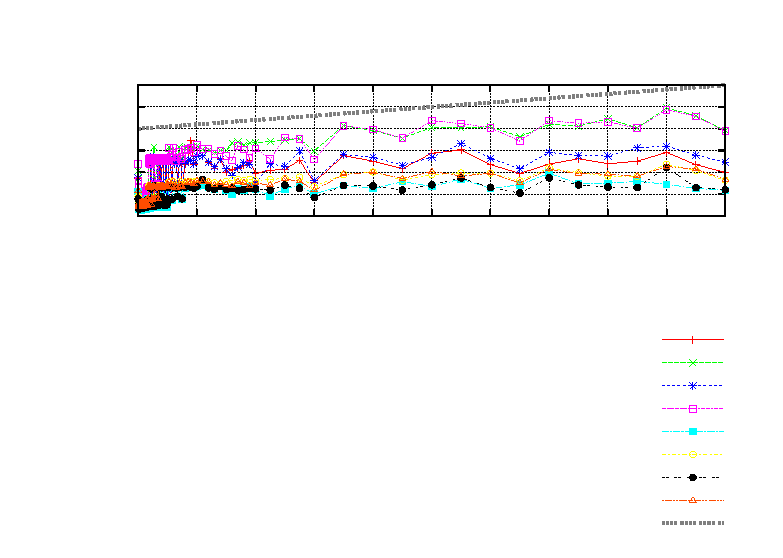
\includegraphics{ej3_nodos_wheel}}%
    \gplfronttext
  \end{picture}%
\endgroup
}
    \caption{Complejidad temporal para Ruedas}
\end{figure}

\begin{figure}[H]
    \centering
    \fontsize{7}{10}\selectfont
    \resizebox{0.8\textwidth}{!}{% GNUPLOT: LaTeX picture with Postscript
\begingroup
  \makeatletter
  \providecommand\color[2][]{%
    \GenericError{(gnuplot) \space\space\space\@spaces}{%
      Package color not loaded in conjunction with
      terminal option `colourtext'%
    }{See the gnuplot documentation for explanation.%
    }{Either use 'blacktext' in gnuplot or load the package
      color.sty in LaTeX.}%
    \renewcommand\color[2][]{}%
  }%
  \providecommand\includegraphics[2][]{%
    \GenericError{(gnuplot) \space\space\space\@spaces}{%
      Package graphicx or graphics not loaded%
    }{See the gnuplot documentation for explanation.%
    }{The gnuplot epslatex terminal needs graphicx.sty or graphics.sty.}%
    \renewcommand\includegraphics[2][]{}%
  }%
  \providecommand\rotatebox[2]{#2}%
  \@ifundefined{ifGPcolor}{%
    \newif\ifGPcolor
    \GPcolortrue
  }{}%
  \@ifundefined{ifGPblacktext}{%
    \newif\ifGPblacktext
    \GPblacktexttrue
  }{}%
  % define a \g@addto@macro without @ in the name:
  \let\gplgaddtomacro\g@addto@macro
  % define empty templates for all commands taking text:
  \gdef\gplbacktext{}%
  \gdef\gplfronttext{}%
  \makeatother
  \ifGPblacktext
    % no textcolor at all
    \def\colorrgb#1{}%
    \def\colorgray#1{}%
  \else
    % gray or color?
    \ifGPcolor
      \def\colorrgb#1{\color[rgb]{#1}}%
      \def\colorgray#1{\color[gray]{#1}}%
      \expandafter\def\csname LTw\endcsname{\color{white}}%
      \expandafter\def\csname LTb\endcsname{\color{black}}%
      \expandafter\def\csname LTa\endcsname{\color{black}}%
      \expandafter\def\csname LT0\endcsname{\color[rgb]{1,0,0}}%
      \expandafter\def\csname LT1\endcsname{\color[rgb]{0,1,0}}%
      \expandafter\def\csname LT2\endcsname{\color[rgb]{0,0,1}}%
      \expandafter\def\csname LT3\endcsname{\color[rgb]{1,0,1}}%
      \expandafter\def\csname LT4\endcsname{\color[rgb]{0,1,1}}%
      \expandafter\def\csname LT5\endcsname{\color[rgb]{1,1,0}}%
      \expandafter\def\csname LT6\endcsname{\color[rgb]{0,0,0}}%
      \expandafter\def\csname LT7\endcsname{\color[rgb]{1,0.3,0}}%
      \expandafter\def\csname LT8\endcsname{\color[rgb]{0.5,0.5,0.5}}%
    \else
      % gray
      \def\colorrgb#1{\color{black}}%
      \def\colorgray#1{\color[gray]{#1}}%
      \expandafter\def\csname LTw\endcsname{\color{white}}%
      \expandafter\def\csname LTb\endcsname{\color{black}}%
      \expandafter\def\csname LTa\endcsname{\color{black}}%
      \expandafter\def\csname LT0\endcsname{\color{black}}%
      \expandafter\def\csname LT1\endcsname{\color{black}}%
      \expandafter\def\csname LT2\endcsname{\color{black}}%
      \expandafter\def\csname LT3\endcsname{\color{black}}%
      \expandafter\def\csname LT4\endcsname{\color{black}}%
      \expandafter\def\csname LT5\endcsname{\color{black}}%
      \expandafter\def\csname LT6\endcsname{\color{black}}%
      \expandafter\def\csname LT7\endcsname{\color{black}}%
      \expandafter\def\csname LT8\endcsname{\color{black}}%
    \fi
  \fi
  \setlength{\unitlength}{0.0500bp}%
  \begin{picture}(7200.00,5040.00)%
    \gplgaddtomacro\gplbacktext{%
      \csname LTb\endcsname%
      \put(1430,2904){\makebox(0,0)[r]{\strut{} 0}}%
      \csname LTb\endcsname%
      \put(1430,3052){\makebox(0,0)[r]{\strut{} 1000}}%
      \csname LTb\endcsname%
      \put(1430,3199){\makebox(0,0)[r]{\strut{} 2000}}%
      \csname LTb\endcsname%
      \put(1430,3347){\makebox(0,0)[r]{\strut{} 3000}}%
      \csname LTb\endcsname%
      \put(1430,3494){\makebox(0,0)[r]{\strut{} 4000}}%
      \csname LTb\endcsname%
      \put(1430,3642){\makebox(0,0)[r]{\strut{} 5000}}%
      \csname LTb\endcsname%
      \put(1430,3789){\makebox(0,0)[r]{\strut{} 6000}}%
      \csname LTb\endcsname%
      \put(1430,3937){\makebox(0,0)[r]{\strut{} 7000}}%
      \csname LTb\endcsname%
      \put(1430,4084){\makebox(0,0)[r]{\strut{} 8000}}%
      \csname LTb\endcsname%
      \put(1430,4232){\makebox(0,0)[r]{\strut{} 9000}}%
      \csname LTb\endcsname%
      \put(1430,4379){\makebox(0,0)[r]{\strut{} 10000}}%
      \csname LTb\endcsname%
      \put(1562,2684){\makebox(0,0){\strut{} 0}}%
      \csname LTb\endcsname%
      \put(2086,2684){\makebox(0,0){\strut{} 1000}}%
      \csname LTb\endcsname%
      \put(2610,2684){\makebox(0,0){\strut{} 2000}}%
      \csname LTb\endcsname%
      \put(3134,2684){\makebox(0,0){\strut{} 3000}}%
      \csname LTb\endcsname%
      \put(3658,2684){\makebox(0,0){\strut{} 4000}}%
      \csname LTb\endcsname%
      \put(4183,2684){\makebox(0,0){\strut{} 5000}}%
      \csname LTb\endcsname%
      \put(4707,2684){\makebox(0,0){\strut{} 6000}}%
      \csname LTb\endcsname%
      \put(5231,2684){\makebox(0,0){\strut{} 7000}}%
      \csname LTb\endcsname%
      \put(5755,2684){\makebox(0,0){\strut{} 8000}}%
      \csname LTb\endcsname%
      \put(6279,2684){\makebox(0,0){\strut{} 9000}}%
      \csname LTb\endcsname%
      \put(6803,2684){\makebox(0,0){\strut{} 10000}}%
      \put(176,3641){\rotatebox{-270}{\makebox(0,0){\strut{}Frontera}}}%
      \put(396,3641){\rotatebox{-270}{\makebox(0,0){\strut{}(Escala Lineal)}}}%
      \put(4182,2354){\makebox(0,0){\strut{}Cantidad de Nodos}}%
      \put(4182,2134){\makebox(0,0){\strut{}(Escala Lineal)}}%
      \put(4182,4709){\makebox(0,0){\strut{}Relacion Frontera/Nodos}}%
    }%
    \gplgaddtomacro\gplfronttext{%
      \csname LTb\endcsname%
      \put(6263,1713){\makebox(0,0)[r]{\strut{}Primer Vecino}}%
      \csname LTb\endcsname%
      \put(6263,1493){\makebox(0,0)[r]{\strut{}Primer Vecino con golosa}}%
      \csname LTb\endcsname%
      \put(6263,1273){\makebox(0,0)[r]{\strut{}Primer Vecino con intercambio}}%
      \csname LTb\endcsname%
      \put(6263,1053){\makebox(0,0)[r]{\strut{}Primer Vecino con intercambio y golosa}}%
      \csname LTb\endcsname%
      \put(6263,833){\makebox(0,0)[r]{\strut{}Mejor Vecino}}%
      \csname LTb\endcsname%
      \put(6263,613){\makebox(0,0)[r]{\strut{}Mejor Vecino con golosa}}%
      \csname LTb\endcsname%
      \put(6263,393){\makebox(0,0)[r]{\strut{}Mejor Vecino con intercambio}}%
      \csname LTb\endcsname%
      \put(6263,173){\makebox(0,0)[r]{\strut{}Mejor Vecino con intercambio y golosa}}%
    }%
    \gplbacktext
    \put(0,0){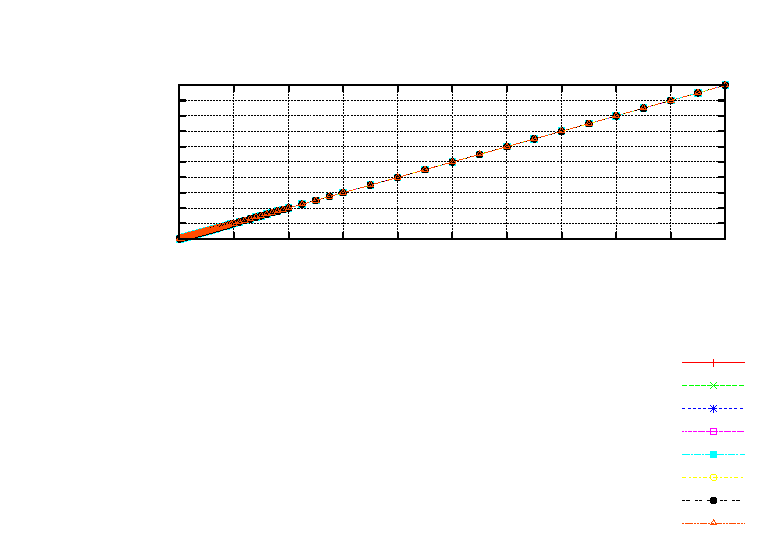
\includegraphics{ej3_frontera_wheel}}%
    \gplfronttext
  \end{picture}%
\endgroup
}
    \caption{Frontera para Ruedas}
\end{figure}

\bigskip

\par Como ya se ha explicado, para esta familia tenemos la certeza te\'orica de que
    nuestra heur\'istica propuesta resolver\'a el problema de manera \'optima (sin
    importar la variante). Es bueno confirmar dicha proposici\'on (parcialmente) emp\'iricamente,
    como se puede observar en el grafico de ``Frontera'' obtenida. En realidad se observa
    que todas las variantes dan el mismo resultado. Falta comprobar que este sea el correcto,
    cosa que se puede an\'alizar con los resultados del algoritmo exacto ya implementado%
    \footnote{Dicho an\'alisis no se realiz\'o por falta de tiempo.}.

\par Tambi\'en, haciendo hincapi\'e en los resultados de complejidad temporal,
    nuevamente se destaca que la variante \emph{Mejor Vecino con Intercambio}
    es una de las implementaciones que menos tiempo requiere (y como todas las
    dem\'as, da la misma respuesta). En sinton\'ia con esto, se observa
    que las variantes que realizan saltos de mayor calidad dentro de la vecindad
    requieren menos tiempo para terminar (en el contexto de esta familia de grafos).

%Circulares
\begin{figure}[H]
    \centering
    \fontsize{7}{10}\selectfont
    \resizebox{0.8\textwidth}{!}{% GNUPLOT: LaTeX picture with Postscript
\begingroup
  \makeatletter
  \providecommand\color[2][]{%
    \GenericError{(gnuplot) \space\space\space\@spaces}{%
      Package color not loaded in conjunction with
      terminal option `colourtext'%
    }{See the gnuplot documentation for explanation.%
    }{Either use 'blacktext' in gnuplot or load the package
      color.sty in LaTeX.}%
    \renewcommand\color[2][]{}%
  }%
  \providecommand\includegraphics[2][]{%
    \GenericError{(gnuplot) \space\space\space\@spaces}{%
      Package graphicx or graphics not loaded%
    }{See the gnuplot documentation for explanation.%
    }{The gnuplot epslatex terminal needs graphicx.sty or graphics.sty.}%
    \renewcommand\includegraphics[2][]{}%
  }%
  \providecommand\rotatebox[2]{#2}%
  \@ifundefined{ifGPcolor}{%
    \newif\ifGPcolor
    \GPcolortrue
  }{}%
  \@ifundefined{ifGPblacktext}{%
    \newif\ifGPblacktext
    \GPblacktexttrue
  }{}%
  % define a \g@addto@macro without @ in the name:
  \let\gplgaddtomacro\g@addto@macro
  % define empty templates for all commands taking text:
  \gdef\gplbacktext{}%
  \gdef\gplfronttext{}%
  \makeatother
  \ifGPblacktext
    % no textcolor at all
    \def\colorrgb#1{}%
    \def\colorgray#1{}%
  \else
    % gray or color?
    \ifGPcolor
      \def\colorrgb#1{\color[rgb]{#1}}%
      \def\colorgray#1{\color[gray]{#1}}%
      \expandafter\def\csname LTw\endcsname{\color{white}}%
      \expandafter\def\csname LTb\endcsname{\color{black}}%
      \expandafter\def\csname LTa\endcsname{\color{black}}%
      \expandafter\def\csname LT0\endcsname{\color[rgb]{1,0,0}}%
      \expandafter\def\csname LT1\endcsname{\color[rgb]{0,1,0}}%
      \expandafter\def\csname LT2\endcsname{\color[rgb]{0,0,1}}%
      \expandafter\def\csname LT3\endcsname{\color[rgb]{1,0,1}}%
      \expandafter\def\csname LT4\endcsname{\color[rgb]{0,1,1}}%
      \expandafter\def\csname LT5\endcsname{\color[rgb]{1,1,0}}%
      \expandafter\def\csname LT6\endcsname{\color[rgb]{0,0,0}}%
      \expandafter\def\csname LT7\endcsname{\color[rgb]{1,0.3,0}}%
      \expandafter\def\csname LT8\endcsname{\color[rgb]{0.5,0.5,0.5}}%
    \else
      % gray
      \def\colorrgb#1{\color{black}}%
      \def\colorgray#1{\color[gray]{#1}}%
      \expandafter\def\csname LTw\endcsname{\color{white}}%
      \expandafter\def\csname LTb\endcsname{\color{black}}%
      \expandafter\def\csname LTa\endcsname{\color{black}}%
      \expandafter\def\csname LT0\endcsname{\color{black}}%
      \expandafter\def\csname LT1\endcsname{\color{black}}%
      \expandafter\def\csname LT2\endcsname{\color{black}}%
      \expandafter\def\csname LT3\endcsname{\color{black}}%
      \expandafter\def\csname LT4\endcsname{\color{black}}%
      \expandafter\def\csname LT5\endcsname{\color{black}}%
      \expandafter\def\csname LT6\endcsname{\color{black}}%
      \expandafter\def\csname LT7\endcsname{\color{black}}%
      \expandafter\def\csname LT8\endcsname{\color{black}}%
    \fi
  \fi
  \setlength{\unitlength}{0.0500bp}%
  \begin{picture}(7200.00,5040.00)%
    \gplgaddtomacro\gplbacktext{%
      \csname LTb\endcsname%
      \put(1034,3124){\makebox(0,0)[r]{\strut{} 0}}%
      \csname LTb\endcsname%
      \put(1034,3333){\makebox(0,0)[r]{\strut{} 10}}%
      \csname LTb\endcsname%
      \put(1034,3542){\makebox(0,0)[r]{\strut{} 20}}%
      \csname LTb\endcsname%
      \put(1034,3752){\makebox(0,0)[r]{\strut{} 30}}%
      \csname LTb\endcsname%
      \put(1034,3961){\makebox(0,0)[r]{\strut{} 40}}%
      \csname LTb\endcsname%
      \put(1034,4170){\makebox(0,0)[r]{\strut{} 50}}%
      \csname LTb\endcsname%
      \put(1034,4379){\makebox(0,0)[r]{\strut{} 60}}%
      \csname LTb\endcsname%
      \put(1166,2904){\makebox(0,0){\strut{} 0}}%
      \csname LTb\endcsname%
      \put(1730,2904){\makebox(0,0){\strut{} 1000}}%
      \csname LTb\endcsname%
      \put(2293,2904){\makebox(0,0){\strut{} 2000}}%
      \csname LTb\endcsname%
      \put(2857,2904){\makebox(0,0){\strut{} 3000}}%
      \csname LTb\endcsname%
      \put(3421,2904){\makebox(0,0){\strut{} 4000}}%
      \csname LTb\endcsname%
      \put(3985,2904){\makebox(0,0){\strut{} 5000}}%
      \csname LTb\endcsname%
      \put(4548,2904){\makebox(0,0){\strut{} 6000}}%
      \csname LTb\endcsname%
      \put(5112,2904){\makebox(0,0){\strut{} 7000}}%
      \csname LTb\endcsname%
      \put(5676,2904){\makebox(0,0){\strut{} 8000}}%
      \csname LTb\endcsname%
      \put(6239,2904){\makebox(0,0){\strut{} 9000}}%
      \csname LTb\endcsname%
      \put(6803,2904){\makebox(0,0){\strut{} 10000}}%
      \put(176,3751){\rotatebox{-270}{\makebox(0,0){\strut{}Tiempo ($nanosegundos^{\sfrac{1}{5}}$)}}}%
      \put(396,3751){\rotatebox{-270}{\makebox(0,0){\strut{}(Escala Lineal)}}}%
      \put(3984,2574){\makebox(0,0){\strut{}Cantidad de Nodos}}%
      \put(3984,2354){\makebox(0,0){\strut{}(Escala Lineal)}}%
      \put(3984,4709){\makebox(0,0){\strut{}Tiempo de ejecución conforme aumenta la cantidad de nodos}}%
    }%
    \gplgaddtomacro\gplfronttext{%
      \csname LTb\endcsname%
      \put(6065,1933){\makebox(0,0)[r]{\strut{}Primer Vecino}}%
      \csname LTb\endcsname%
      \put(6065,1713){\makebox(0,0)[r]{\strut{}Primer Vecino con golosa}}%
      \csname LTb\endcsname%
      \put(6065,1493){\makebox(0,0)[r]{\strut{}Primer Vecino con intercambio}}%
      \csname LTb\endcsname%
      \put(6065,1273){\makebox(0,0)[r]{\strut{}Primer Vecino con intercambio y golosa}}%
      \csname LTb\endcsname%
      \put(6065,1053){\makebox(0,0)[r]{\strut{}Mejor Vecino}}%
      \csname LTb\endcsname%
      \put(6065,833){\makebox(0,0)[r]{\strut{}Mejor Vecino con golosa}}%
      \csname LTb\endcsname%
      \put(6065,613){\makebox(0,0)[r]{\strut{}Mejor Vecino con intercambio}}%
      \csname LTb\endcsname%
      \put(6065,393){\makebox(0,0)[r]{\strut{}Mejor Vecino con intercambio y golosa}}%
      \csname LTb\endcsname%
      \put(6065,173){\makebox(0,0)[r]{\strut{}Cota teórica superior $\mathcal O(n)$}}%
    }%
    \gplbacktext
    \put(0,0){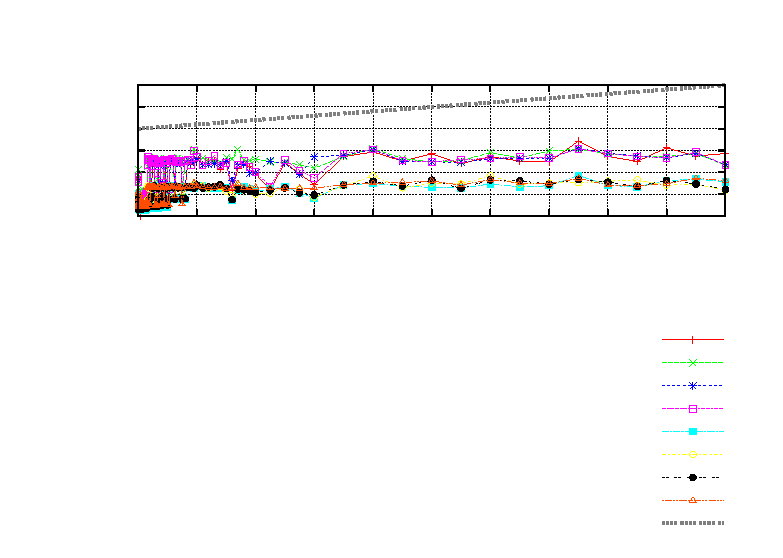
\includegraphics{ej3_nodos_hole}}%
    \gplfronttext
  \end{picture}%
\endgroup
}
    \caption{Complejidad temporal para grafos Circulares}
\end{figure}

\begin{figure}[H]
    \centering
    \fontsize{7}{10}\selectfont
    \resizebox{0.8\textwidth}{!}{% GNUPLOT: LaTeX picture with Postscript
\begingroup
  \makeatletter
  \providecommand\color[2][]{%
    \GenericError{(gnuplot) \space\space\space\@spaces}{%
      Package color not loaded in conjunction with
      terminal option `colourtext'%
    }{See the gnuplot documentation for explanation.%
    }{Either use 'blacktext' in gnuplot or load the package
      color.sty in LaTeX.}%
    \renewcommand\color[2][]{}%
  }%
  \providecommand\includegraphics[2][]{%
    \GenericError{(gnuplot) \space\space\space\@spaces}{%
      Package graphicx or graphics not loaded%
    }{See the gnuplot documentation for explanation.%
    }{The gnuplot epslatex terminal needs graphicx.sty or graphics.sty.}%
    \renewcommand\includegraphics[2][]{}%
  }%
  \providecommand\rotatebox[2]{#2}%
  \@ifundefined{ifGPcolor}{%
    \newif\ifGPcolor
    \GPcolortrue
  }{}%
  \@ifundefined{ifGPblacktext}{%
    \newif\ifGPblacktext
    \GPblacktexttrue
  }{}%
  % define a \g@addto@macro without @ in the name:
  \let\gplgaddtomacro\g@addto@macro
  % define empty templates for all commands taking text:
  \gdef\gplbacktext{}%
  \gdef\gplfronttext{}%
  \makeatother
  \ifGPblacktext
    % no textcolor at all
    \def\colorrgb#1{}%
    \def\colorgray#1{}%
  \else
    % gray or color?
    \ifGPcolor
      \def\colorrgb#1{\color[rgb]{#1}}%
      \def\colorgray#1{\color[gray]{#1}}%
      \expandafter\def\csname LTw\endcsname{\color{white}}%
      \expandafter\def\csname LTb\endcsname{\color{black}}%
      \expandafter\def\csname LTa\endcsname{\color{black}}%
      \expandafter\def\csname LT0\endcsname{\color[rgb]{1,0,0}}%
      \expandafter\def\csname LT1\endcsname{\color[rgb]{0,1,0}}%
      \expandafter\def\csname LT2\endcsname{\color[rgb]{0,0,1}}%
      \expandafter\def\csname LT3\endcsname{\color[rgb]{1,0,1}}%
      \expandafter\def\csname LT4\endcsname{\color[rgb]{0,1,1}}%
      \expandafter\def\csname LT5\endcsname{\color[rgb]{1,1,0}}%
      \expandafter\def\csname LT6\endcsname{\color[rgb]{0,0,0}}%
      \expandafter\def\csname LT7\endcsname{\color[rgb]{1,0.3,0}}%
      \expandafter\def\csname LT8\endcsname{\color[rgb]{0.5,0.5,0.5}}%
    \else
      % gray
      \def\colorrgb#1{\color{black}}%
      \def\colorgray#1{\color[gray]{#1}}%
      \expandafter\def\csname LTw\endcsname{\color{white}}%
      \expandafter\def\csname LTb\endcsname{\color{black}}%
      \expandafter\def\csname LTa\endcsname{\color{black}}%
      \expandafter\def\csname LT0\endcsname{\color{black}}%
      \expandafter\def\csname LT1\endcsname{\color{black}}%
      \expandafter\def\csname LT2\endcsname{\color{black}}%
      \expandafter\def\csname LT3\endcsname{\color{black}}%
      \expandafter\def\csname LT4\endcsname{\color{black}}%
      \expandafter\def\csname LT5\endcsname{\color{black}}%
      \expandafter\def\csname LT6\endcsname{\color{black}}%
      \expandafter\def\csname LT7\endcsname{\color{black}}%
      \expandafter\def\csname LT8\endcsname{\color{black}}%
    \fi
  \fi
  \setlength{\unitlength}{0.0500bp}%
  \begin{picture}(7200.00,5040.00)%
    \gplgaddtomacro\gplbacktext{%
      \csname LTb\endcsname%
      \put(1430,2904){\makebox(0,0)[r]{\strut{} 1.98}}%
      \csname LTb\endcsname%
      \put(1430,3088){\makebox(0,0)[r]{\strut{} 1.985}}%
      \csname LTb\endcsname%
      \put(1430,3273){\makebox(0,0)[r]{\strut{} 1.99}}%
      \csname LTb\endcsname%
      \put(1430,3457){\makebox(0,0)[r]{\strut{} 1.995}}%
      \csname LTb\endcsname%
      \put(1430,3641){\makebox(0,0)[r]{\strut{} 2}}%
      \csname LTb\endcsname%
      \put(1430,3826){\makebox(0,0)[r]{\strut{} 2.005}}%
      \csname LTb\endcsname%
      \put(1430,4010){\makebox(0,0)[r]{\strut{} 2.01}}%
      \csname LTb\endcsname%
      \put(1430,4195){\makebox(0,0)[r]{\strut{} 2.015}}%
      \csname LTb\endcsname%
      \put(1430,4379){\makebox(0,0)[r]{\strut{} 2.02}}%
      \csname LTb\endcsname%
      \put(1562,2684){\makebox(0,0){\strut{} 0}}%
      \csname LTb\endcsname%
      \put(2086,2684){\makebox(0,0){\strut{} 1000}}%
      \csname LTb\endcsname%
      \put(2610,2684){\makebox(0,0){\strut{} 2000}}%
      \csname LTb\endcsname%
      \put(3134,2684){\makebox(0,0){\strut{} 3000}}%
      \csname LTb\endcsname%
      \put(3658,2684){\makebox(0,0){\strut{} 4000}}%
      \csname LTb\endcsname%
      \put(4183,2684){\makebox(0,0){\strut{} 5000}}%
      \csname LTb\endcsname%
      \put(4707,2684){\makebox(0,0){\strut{} 6000}}%
      \csname LTb\endcsname%
      \put(5231,2684){\makebox(0,0){\strut{} 7000}}%
      \csname LTb\endcsname%
      \put(5755,2684){\makebox(0,0){\strut{} 8000}}%
      \csname LTb\endcsname%
      \put(6279,2684){\makebox(0,0){\strut{} 9000}}%
      \csname LTb\endcsname%
      \put(6803,2684){\makebox(0,0){\strut{} 10000}}%
      \put(176,3641){\rotatebox{-270}{\makebox(0,0){\strut{}Frontera}}}%
      \put(396,3641){\rotatebox{-270}{\makebox(0,0){\strut{}(Escala Lineal)}}}%
      \put(4182,2354){\makebox(0,0){\strut{}Cantidad de Nodos}}%
      \put(4182,2134){\makebox(0,0){\strut{}(Escala Lineal)}}%
      \put(4182,4709){\makebox(0,0){\strut{}Relacion Frontera/Nodos}}%
    }%
    \gplgaddtomacro\gplfronttext{%
      \csname LTb\endcsname%
      \put(6263,1713){\makebox(0,0)[r]{\strut{}Primer Vecino}}%
      \csname LTb\endcsname%
      \put(6263,1493){\makebox(0,0)[r]{\strut{}Primer Vecino con golosa}}%
      \csname LTb\endcsname%
      \put(6263,1273){\makebox(0,0)[r]{\strut{}Primer Vecino con intercambio}}%
      \csname LTb\endcsname%
      \put(6263,1053){\makebox(0,0)[r]{\strut{}Primer Vecino con intercambio y golosa}}%
      \csname LTb\endcsname%
      \put(6263,833){\makebox(0,0)[r]{\strut{}Mejor Vecino}}%
      \csname LTb\endcsname%
      \put(6263,613){\makebox(0,0)[r]{\strut{}Mejor Vecino con golosa}}%
      \csname LTb\endcsname%
      \put(6263,393){\makebox(0,0)[r]{\strut{}Mejor Vecino con intercambio}}%
      \csname LTb\endcsname%
      \put(6263,173){\makebox(0,0)[r]{\strut{}Mejor Vecino con intercambio y golosa}}%
    }%
    \gplbacktext
    \put(0,0){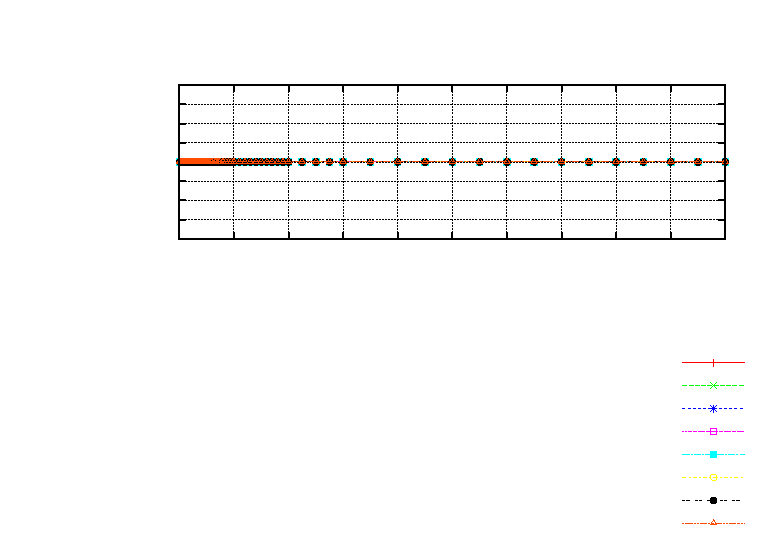
\includegraphics{ej3_frontera_hole}}%
    \gplfronttext
  \end{picture}%
\endgroup
}
    \caption{Fronteras para grafos Circulares}
\end{figure}

%Estrella
\begin{figure}[H]
    \centering
    \fontsize{7}{10}\selectfont
    \resizebox{0.8\textwidth}{!}{% GNUPLOT: LaTeX picture with Postscript
\begingroup
  \makeatletter
  \providecommand\color[2][]{%
    \GenericError{(gnuplot) \space\space\space\@spaces}{%
      Package color not loaded in conjunction with
      terminal option `colourtext'%
    }{See the gnuplot documentation for explanation.%
    }{Either use 'blacktext' in gnuplot or load the package
      color.sty in LaTeX.}%
    \renewcommand\color[2][]{}%
  }%
  \providecommand\includegraphics[2][]{%
    \GenericError{(gnuplot) \space\space\space\@spaces}{%
      Package graphicx or graphics not loaded%
    }{See the gnuplot documentation for explanation.%
    }{The gnuplot epslatex terminal needs graphicx.sty or graphics.sty.}%
    \renewcommand\includegraphics[2][]{}%
  }%
  \providecommand\rotatebox[2]{#2}%
  \@ifundefined{ifGPcolor}{%
    \newif\ifGPcolor
    \GPcolortrue
  }{}%
  \@ifundefined{ifGPblacktext}{%
    \newif\ifGPblacktext
    \GPblacktexttrue
  }{}%
  % define a \g@addto@macro without @ in the name:
  \let\gplgaddtomacro\g@addto@macro
  % define empty templates for all commands taking text:
  \gdef\gplbacktext{}%
  \gdef\gplfronttext{}%
  \makeatother
  \ifGPblacktext
    % no textcolor at all
    \def\colorrgb#1{}%
    \def\colorgray#1{}%
  \else
    % gray or color?
    \ifGPcolor
      \def\colorrgb#1{\color[rgb]{#1}}%
      \def\colorgray#1{\color[gray]{#1}}%
      \expandafter\def\csname LTw\endcsname{\color{white}}%
      \expandafter\def\csname LTb\endcsname{\color{black}}%
      \expandafter\def\csname LTa\endcsname{\color{black}}%
      \expandafter\def\csname LT0\endcsname{\color[rgb]{1,0,0}}%
      \expandafter\def\csname LT1\endcsname{\color[rgb]{0,1,0}}%
      \expandafter\def\csname LT2\endcsname{\color[rgb]{0,0,1}}%
      \expandafter\def\csname LT3\endcsname{\color[rgb]{1,0,1}}%
      \expandafter\def\csname LT4\endcsname{\color[rgb]{0,1,1}}%
      \expandafter\def\csname LT5\endcsname{\color[rgb]{1,1,0}}%
      \expandafter\def\csname LT6\endcsname{\color[rgb]{0,0,0}}%
      \expandafter\def\csname LT7\endcsname{\color[rgb]{1,0.3,0}}%
      \expandafter\def\csname LT8\endcsname{\color[rgb]{0.5,0.5,0.5}}%
    \else
      % gray
      \def\colorrgb#1{\color{black}}%
      \def\colorgray#1{\color[gray]{#1}}%
      \expandafter\def\csname LTw\endcsname{\color{white}}%
      \expandafter\def\csname LTb\endcsname{\color{black}}%
      \expandafter\def\csname LTa\endcsname{\color{black}}%
      \expandafter\def\csname LT0\endcsname{\color{black}}%
      \expandafter\def\csname LT1\endcsname{\color{black}}%
      \expandafter\def\csname LT2\endcsname{\color{black}}%
      \expandafter\def\csname LT3\endcsname{\color{black}}%
      \expandafter\def\csname LT4\endcsname{\color{black}}%
      \expandafter\def\csname LT5\endcsname{\color{black}}%
      \expandafter\def\csname LT6\endcsname{\color{black}}%
      \expandafter\def\csname LT7\endcsname{\color{black}}%
      \expandafter\def\csname LT8\endcsname{\color{black}}%
    \fi
  \fi
  \setlength{\unitlength}{0.0500bp}%
  \begin{picture}(7200.00,5040.00)%
    \gplgaddtomacro\gplbacktext{%
      \csname LTb\endcsname%
      \put(1034,3124){\makebox(0,0)[r]{\strut{} 0}}%
      \csname LTb\endcsname%
      \put(1034,3333){\makebox(0,0)[r]{\strut{} 10}}%
      \csname LTb\endcsname%
      \put(1034,3542){\makebox(0,0)[r]{\strut{} 20}}%
      \csname LTb\endcsname%
      \put(1034,3752){\makebox(0,0)[r]{\strut{} 30}}%
      \csname LTb\endcsname%
      \put(1034,3961){\makebox(0,0)[r]{\strut{} 40}}%
      \csname LTb\endcsname%
      \put(1034,4170){\makebox(0,0)[r]{\strut{} 50}}%
      \csname LTb\endcsname%
      \put(1034,4379){\makebox(0,0)[r]{\strut{} 60}}%
      \csname LTb\endcsname%
      \put(1166,2904){\makebox(0,0){\strut{} 0}}%
      \csname LTb\endcsname%
      \put(1730,2904){\makebox(0,0){\strut{} 1000}}%
      \csname LTb\endcsname%
      \put(2293,2904){\makebox(0,0){\strut{} 2000}}%
      \csname LTb\endcsname%
      \put(2857,2904){\makebox(0,0){\strut{} 3000}}%
      \csname LTb\endcsname%
      \put(3421,2904){\makebox(0,0){\strut{} 4000}}%
      \csname LTb\endcsname%
      \put(3985,2904){\makebox(0,0){\strut{} 5000}}%
      \csname LTb\endcsname%
      \put(4548,2904){\makebox(0,0){\strut{} 6000}}%
      \csname LTb\endcsname%
      \put(5112,2904){\makebox(0,0){\strut{} 7000}}%
      \csname LTb\endcsname%
      \put(5676,2904){\makebox(0,0){\strut{} 8000}}%
      \csname LTb\endcsname%
      \put(6239,2904){\makebox(0,0){\strut{} 9000}}%
      \csname LTb\endcsname%
      \put(6803,2904){\makebox(0,0){\strut{} 10000}}%
      \put(176,3751){\rotatebox{-270}{\makebox(0,0){\strut{}Tiempo ($nanosegundos^{\sfrac{1}{5}}$)}}}%
      \put(396,3751){\rotatebox{-270}{\makebox(0,0){\strut{}(Escala Lineal)}}}%
      \put(3984,2574){\makebox(0,0){\strut{}Cantidad de Nodos}}%
      \put(3984,2354){\makebox(0,0){\strut{}(Escala Lineal)}}%
      \put(3984,4709){\makebox(0,0){\strut{}Tiempo de ejecución conforme aumenta la cantidad de nodos}}%
    }%
    \gplgaddtomacro\gplfronttext{%
      \csname LTb\endcsname%
      \put(6065,1933){\makebox(0,0)[r]{\strut{}Primer Vecino}}%
      \csname LTb\endcsname%
      \put(6065,1713){\makebox(0,0)[r]{\strut{}Primer Vecino con golosa}}%
      \csname LTb\endcsname%
      \put(6065,1493){\makebox(0,0)[r]{\strut{}Primer Vecino con intercambio}}%
      \csname LTb\endcsname%
      \put(6065,1273){\makebox(0,0)[r]{\strut{}Primer Vecino con intercambio y golosa}}%
      \csname LTb\endcsname%
      \put(6065,1053){\makebox(0,0)[r]{\strut{}Mejor Vecino}}%
      \csname LTb\endcsname%
      \put(6065,833){\makebox(0,0)[r]{\strut{}Mejor Vecino con golosa}}%
      \csname LTb\endcsname%
      \put(6065,613){\makebox(0,0)[r]{\strut{}Mejor Vecino con intercambio}}%
      \csname LTb\endcsname%
      \put(6065,393){\makebox(0,0)[r]{\strut{}Mejor Vecino con intercambio y golosa}}%
      \csname LTb\endcsname%
      \put(6065,173){\makebox(0,0)[r]{\strut{}Cota teórica superior $\mathcal O(n)$}}%
    }%
    \gplbacktext
    \put(0,0){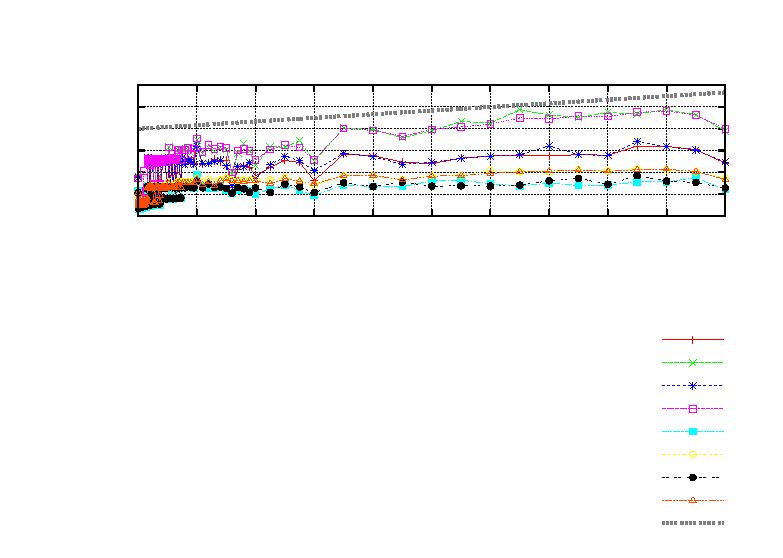
\includegraphics{ej3_nodos_star}}%
    \gplfronttext
  \end{picture}%
\endgroup
}
    \caption{Complejidad temporal para Estrellas}
\end{figure}

\begin{figure}[H]
    \centering
    \fontsize{7}{10}\selectfont
    \resizebox{0.8\textwidth}{!}{% GNUPLOT: LaTeX picture with Postscript
\begingroup
  \makeatletter
  \providecommand\color[2][]{%
    \GenericError{(gnuplot) \space\space\space\@spaces}{%
      Package color not loaded in conjunction with
      terminal option `colourtext'%
    }{See the gnuplot documentation for explanation.%
    }{Either use 'blacktext' in gnuplot or load the package
      color.sty in LaTeX.}%
    \renewcommand\color[2][]{}%
  }%
  \providecommand\includegraphics[2][]{%
    \GenericError{(gnuplot) \space\space\space\@spaces}{%
      Package graphicx or graphics not loaded%
    }{See the gnuplot documentation for explanation.%
    }{The gnuplot epslatex terminal needs graphicx.sty or graphics.sty.}%
    \renewcommand\includegraphics[2][]{}%
  }%
  \providecommand\rotatebox[2]{#2}%
  \@ifundefined{ifGPcolor}{%
    \newif\ifGPcolor
    \GPcolortrue
  }{}%
  \@ifundefined{ifGPblacktext}{%
    \newif\ifGPblacktext
    \GPblacktexttrue
  }{}%
  % define a \g@addto@macro without @ in the name:
  \let\gplgaddtomacro\g@addto@macro
  % define empty templates for all commands taking text:
  \gdef\gplbacktext{}%
  \gdef\gplfronttext{}%
  \makeatother
  \ifGPblacktext
    % no textcolor at all
    \def\colorrgb#1{}%
    \def\colorgray#1{}%
  \else
    % gray or color?
    \ifGPcolor
      \def\colorrgb#1{\color[rgb]{#1}}%
      \def\colorgray#1{\color[gray]{#1}}%
      \expandafter\def\csname LTw\endcsname{\color{white}}%
      \expandafter\def\csname LTb\endcsname{\color{black}}%
      \expandafter\def\csname LTa\endcsname{\color{black}}%
      \expandafter\def\csname LT0\endcsname{\color[rgb]{1,0,0}}%
      \expandafter\def\csname LT1\endcsname{\color[rgb]{0,1,0}}%
      \expandafter\def\csname LT2\endcsname{\color[rgb]{0,0,1}}%
      \expandafter\def\csname LT3\endcsname{\color[rgb]{1,0,1}}%
      \expandafter\def\csname LT4\endcsname{\color[rgb]{0,1,1}}%
      \expandafter\def\csname LT5\endcsname{\color[rgb]{1,1,0}}%
      \expandafter\def\csname LT6\endcsname{\color[rgb]{0,0,0}}%
      \expandafter\def\csname LT7\endcsname{\color[rgb]{1,0.3,0}}%
      \expandafter\def\csname LT8\endcsname{\color[rgb]{0.5,0.5,0.5}}%
    \else
      % gray
      \def\colorrgb#1{\color{black}}%
      \def\colorgray#1{\color[gray]{#1}}%
      \expandafter\def\csname LTw\endcsname{\color{white}}%
      \expandafter\def\csname LTb\endcsname{\color{black}}%
      \expandafter\def\csname LTa\endcsname{\color{black}}%
      \expandafter\def\csname LT0\endcsname{\color{black}}%
      \expandafter\def\csname LT1\endcsname{\color{black}}%
      \expandafter\def\csname LT2\endcsname{\color{black}}%
      \expandafter\def\csname LT3\endcsname{\color{black}}%
      \expandafter\def\csname LT4\endcsname{\color{black}}%
      \expandafter\def\csname LT5\endcsname{\color{black}}%
      \expandafter\def\csname LT6\endcsname{\color{black}}%
      \expandafter\def\csname LT7\endcsname{\color{black}}%
      \expandafter\def\csname LT8\endcsname{\color{black}}%
    \fi
  \fi
  \setlength{\unitlength}{0.0500bp}%
  \begin{picture}(7200.00,5040.00)%
    \gplgaddtomacro\gplbacktext{%
      \csname LTb\endcsname%
      \put(1430,2904){\makebox(0,0)[r]{\strut{} 0}}%
      \csname LTb\endcsname%
      \put(1430,3052){\makebox(0,0)[r]{\strut{} 1000}}%
      \csname LTb\endcsname%
      \put(1430,3199){\makebox(0,0)[r]{\strut{} 2000}}%
      \csname LTb\endcsname%
      \put(1430,3347){\makebox(0,0)[r]{\strut{} 3000}}%
      \csname LTb\endcsname%
      \put(1430,3494){\makebox(0,0)[r]{\strut{} 4000}}%
      \csname LTb\endcsname%
      \put(1430,3642){\makebox(0,0)[r]{\strut{} 5000}}%
      \csname LTb\endcsname%
      \put(1430,3789){\makebox(0,0)[r]{\strut{} 6000}}%
      \csname LTb\endcsname%
      \put(1430,3937){\makebox(0,0)[r]{\strut{} 7000}}%
      \csname LTb\endcsname%
      \put(1430,4084){\makebox(0,0)[r]{\strut{} 8000}}%
      \csname LTb\endcsname%
      \put(1430,4232){\makebox(0,0)[r]{\strut{} 9000}}%
      \csname LTb\endcsname%
      \put(1430,4379){\makebox(0,0)[r]{\strut{} 10000}}%
      \csname LTb\endcsname%
      \put(1562,2684){\makebox(0,0){\strut{} 0}}%
      \csname LTb\endcsname%
      \put(2086,2684){\makebox(0,0){\strut{} 1000}}%
      \csname LTb\endcsname%
      \put(2610,2684){\makebox(0,0){\strut{} 2000}}%
      \csname LTb\endcsname%
      \put(3134,2684){\makebox(0,0){\strut{} 3000}}%
      \csname LTb\endcsname%
      \put(3658,2684){\makebox(0,0){\strut{} 4000}}%
      \csname LTb\endcsname%
      \put(4183,2684){\makebox(0,0){\strut{} 5000}}%
      \csname LTb\endcsname%
      \put(4707,2684){\makebox(0,0){\strut{} 6000}}%
      \csname LTb\endcsname%
      \put(5231,2684){\makebox(0,0){\strut{} 7000}}%
      \csname LTb\endcsname%
      \put(5755,2684){\makebox(0,0){\strut{} 8000}}%
      \csname LTb\endcsname%
      \put(6279,2684){\makebox(0,0){\strut{} 9000}}%
      \csname LTb\endcsname%
      \put(6803,2684){\makebox(0,0){\strut{} 10000}}%
      \put(176,3641){\rotatebox{-270}{\makebox(0,0){\strut{}Frontera}}}%
      \put(396,3641){\rotatebox{-270}{\makebox(0,0){\strut{}(Escala Lineal)}}}%
      \put(4182,2354){\makebox(0,0){\strut{}Cantidad de Nodos}}%
      \put(4182,2134){\makebox(0,0){\strut{}(Escala Lineal)}}%
      \put(4182,4709){\makebox(0,0){\strut{}Relacion Frontera/Nodos}}%
    }%
    \gplgaddtomacro\gplfronttext{%
      \csname LTb\endcsname%
      \put(6263,1713){\makebox(0,0)[r]{\strut{}Primer Vecino}}%
      \csname LTb\endcsname%
      \put(6263,1493){\makebox(0,0)[r]{\strut{}Primer Vecino con golosa}}%
      \csname LTb\endcsname%
      \put(6263,1273){\makebox(0,0)[r]{\strut{}Primer Vecino con intercambio}}%
      \csname LTb\endcsname%
      \put(6263,1053){\makebox(0,0)[r]{\strut{}Primer Vecino con intercambio y golosa}}%
      \csname LTb\endcsname%
      \put(6263,833){\makebox(0,0)[r]{\strut{}Mejor Vecino}}%
      \csname LTb\endcsname%
      \put(6263,613){\makebox(0,0)[r]{\strut{}Mejor Vecino con golosa}}%
      \csname LTb\endcsname%
      \put(6263,393){\makebox(0,0)[r]{\strut{}Mejor Vecino con intercambio}}%
      \csname LTb\endcsname%
      \put(6263,173){\makebox(0,0)[r]{\strut{}Mejor Vecino con intercambio y golosa}}%
    }%
    \gplbacktext
    \put(0,0){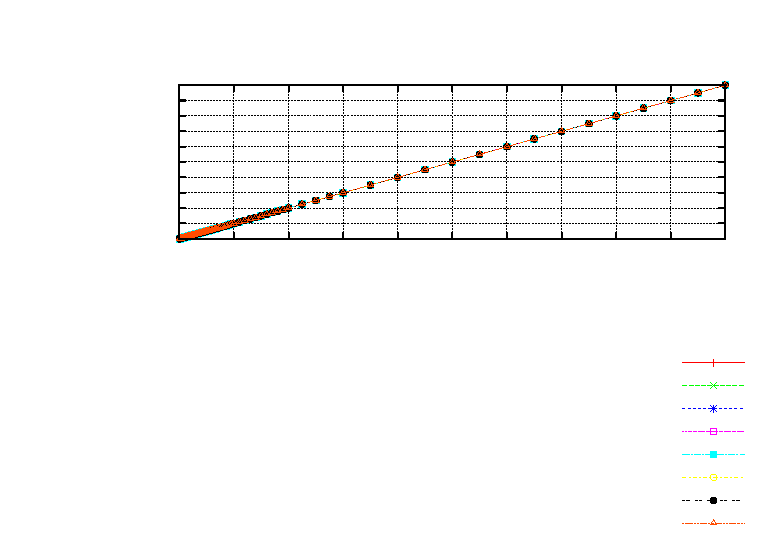
\includegraphics{ej3_frontera_star}}%
    \gplfronttext
  \end{picture}%
\endgroup
}
    \caption{Fronteras para Estrellas}
\end{figure}

%Bipartito
\begin{figure}[H]
    \centering
    \fontsize{7}{10}\selectfont
    \resizebox{0.8\textwidth}{!}{% GNUPLOT: LaTeX picture with Postscript
\begingroup
  \makeatletter
  \providecommand\color[2][]{%
    \GenericError{(gnuplot) \space\space\space\@spaces}{%
      Package color not loaded in conjunction with
      terminal option `colourtext'%
    }{See the gnuplot documentation for explanation.%
    }{Either use 'blacktext' in gnuplot or load the package
      color.sty in LaTeX.}%
    \renewcommand\color[2][]{}%
  }%
  \providecommand\includegraphics[2][]{%
    \GenericError{(gnuplot) \space\space\space\@spaces}{%
      Package graphicx or graphics not loaded%
    }{See the gnuplot documentation for explanation.%
    }{The gnuplot epslatex terminal needs graphicx.sty or graphics.sty.}%
    \renewcommand\includegraphics[2][]{}%
  }%
  \providecommand\rotatebox[2]{#2}%
  \@ifundefined{ifGPcolor}{%
    \newif\ifGPcolor
    \GPcolortrue
  }{}%
  \@ifundefined{ifGPblacktext}{%
    \newif\ifGPblacktext
    \GPblacktexttrue
  }{}%
  % define a \g@addto@macro without @ in the name:
  \let\gplgaddtomacro\g@addto@macro
  % define empty templates for all commands taking text:
  \gdef\gplbacktext{}%
  \gdef\gplfronttext{}%
  \makeatother
  \ifGPblacktext
    % no textcolor at all
    \def\colorrgb#1{}%
    \def\colorgray#1{}%
  \else
    % gray or color?
    \ifGPcolor
      \def\colorrgb#1{\color[rgb]{#1}}%
      \def\colorgray#1{\color[gray]{#1}}%
      \expandafter\def\csname LTw\endcsname{\color{white}}%
      \expandafter\def\csname LTb\endcsname{\color{black}}%
      \expandafter\def\csname LTa\endcsname{\color{black}}%
      \expandafter\def\csname LT0\endcsname{\color[rgb]{1,0,0}}%
      \expandafter\def\csname LT1\endcsname{\color[rgb]{0,1,0}}%
      \expandafter\def\csname LT2\endcsname{\color[rgb]{0,0,1}}%
      \expandafter\def\csname LT3\endcsname{\color[rgb]{1,0,1}}%
      \expandafter\def\csname LT4\endcsname{\color[rgb]{0,1,1}}%
      \expandafter\def\csname LT5\endcsname{\color[rgb]{1,1,0}}%
      \expandafter\def\csname LT6\endcsname{\color[rgb]{0,0,0}}%
      \expandafter\def\csname LT7\endcsname{\color[rgb]{1,0.3,0}}%
      \expandafter\def\csname LT8\endcsname{\color[rgb]{0.5,0.5,0.5}}%
    \else
      % gray
      \def\colorrgb#1{\color{black}}%
      \def\colorgray#1{\color[gray]{#1}}%
      \expandafter\def\csname LTw\endcsname{\color{white}}%
      \expandafter\def\csname LTb\endcsname{\color{black}}%
      \expandafter\def\csname LTa\endcsname{\color{black}}%
      \expandafter\def\csname LT0\endcsname{\color{black}}%
      \expandafter\def\csname LT1\endcsname{\color{black}}%
      \expandafter\def\csname LT2\endcsname{\color{black}}%
      \expandafter\def\csname LT3\endcsname{\color{black}}%
      \expandafter\def\csname LT4\endcsname{\color{black}}%
      \expandafter\def\csname LT5\endcsname{\color{black}}%
      \expandafter\def\csname LT6\endcsname{\color{black}}%
      \expandafter\def\csname LT7\endcsname{\color{black}}%
      \expandafter\def\csname LT8\endcsname{\color{black}}%
    \fi
  \fi
  \setlength{\unitlength}{0.0500bp}%
  \begin{picture}(7200.00,5040.00)%
    \gplgaddtomacro\gplbacktext{%
      \csname LTb\endcsname%
      \put(1034,3124){\makebox(0,0)[r]{\strut{} 0}}%
      \csname LTb\endcsname%
      \put(1034,3250){\makebox(0,0)[r]{\strut{} 5}}%
      \csname LTb\endcsname%
      \put(1034,3375){\makebox(0,0)[r]{\strut{} 10}}%
      \csname LTb\endcsname%
      \put(1034,3501){\makebox(0,0)[r]{\strut{} 15}}%
      \csname LTb\endcsname%
      \put(1034,3626){\makebox(0,0)[r]{\strut{} 20}}%
      \csname LTb\endcsname%
      \put(1034,3752){\makebox(0,0)[r]{\strut{} 25}}%
      \csname LTb\endcsname%
      \put(1034,3877){\makebox(0,0)[r]{\strut{} 30}}%
      \csname LTb\endcsname%
      \put(1034,4003){\makebox(0,0)[r]{\strut{} 35}}%
      \csname LTb\endcsname%
      \put(1034,4128){\makebox(0,0)[r]{\strut{} 40}}%
      \csname LTb\endcsname%
      \put(1034,4254){\makebox(0,0)[r]{\strut{} 45}}%
      \csname LTb\endcsname%
      \put(1034,4379){\makebox(0,0)[r]{\strut{} 50}}%
      \csname LTb\endcsname%
      \put(1166,2904){\makebox(0,0){\strut{} 0}}%
      \csname LTb\endcsname%
      \put(1730,2904){\makebox(0,0){\strut{} 500}}%
      \csname LTb\endcsname%
      \put(2293,2904){\makebox(0,0){\strut{} 1000}}%
      \csname LTb\endcsname%
      \put(2857,2904){\makebox(0,0){\strut{} 1500}}%
      \csname LTb\endcsname%
      \put(3421,2904){\makebox(0,0){\strut{} 2000}}%
      \csname LTb\endcsname%
      \put(3985,2904){\makebox(0,0){\strut{} 2500}}%
      \csname LTb\endcsname%
      \put(4548,2904){\makebox(0,0){\strut{} 3000}}%
      \csname LTb\endcsname%
      \put(5112,2904){\makebox(0,0){\strut{} 3500}}%
      \csname LTb\endcsname%
      \put(5676,2904){\makebox(0,0){\strut{} 4000}}%
      \csname LTb\endcsname%
      \put(6239,2904){\makebox(0,0){\strut{} 4500}}%
      \csname LTb\endcsname%
      \put(6803,2904){\makebox(0,0){\strut{} 5000}}%
      \put(176,3751){\rotatebox{-270}{\makebox(0,0){\strut{}Tiempo ($nanosegundos^{\sfrac{1}{5}}$)}}}%
      \put(396,3751){\rotatebox{-270}{\makebox(0,0){\strut{}(Escala Lineal)}}}%
      \put(3984,2574){\makebox(0,0){\strut{}Cantidad de Nodos}}%
      \put(3984,2354){\makebox(0,0){\strut{}(Escala Lineal)}}%
      \put(3984,4709){\makebox(0,0){\strut{}Tiempo de ejecución conforme aumenta la cantidad de nodos}}%
    }%
    \gplgaddtomacro\gplfronttext{%
      \csname LTb\endcsname%
      \put(6065,1933){\makebox(0,0)[r]{\strut{}Primer Vecino}}%
      \csname LTb\endcsname%
      \put(6065,1713){\makebox(0,0)[r]{\strut{}Primer Vecino con golosa}}%
      \csname LTb\endcsname%
      \put(6065,1493){\makebox(0,0)[r]{\strut{}Primer Vecino con intercambio}}%
      \csname LTb\endcsname%
      \put(6065,1273){\makebox(0,0)[r]{\strut{}Primer Vecino con intercambio y golosa}}%
      \csname LTb\endcsname%
      \put(6065,1053){\makebox(0,0)[r]{\strut{}Mejor Vecino}}%
      \csname LTb\endcsname%
      \put(6065,833){\makebox(0,0)[r]{\strut{}Mejor Vecino con golosa}}%
      \csname LTb\endcsname%
      \put(6065,613){\makebox(0,0)[r]{\strut{}Mejor Vecino con intercambio}}%
      \csname LTb\endcsname%
      \put(6065,393){\makebox(0,0)[r]{\strut{}Mejor Vecino con intercambio y golosa}}%
      \csname LTb\endcsname%
      \put(6065,173){\makebox(0,0)[r]{\strut{}Cota teórica superior $\mathcal O(n)$}}%
    }%
    \gplbacktext
    \put(0,0){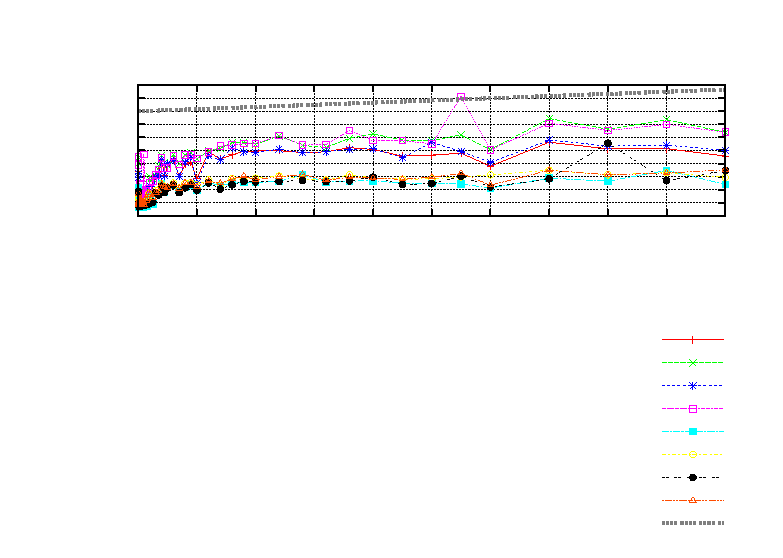
\includegraphics{ej3_nodos_connected_bipartite}}%
    \gplfronttext
  \end{picture}%
\endgroup
}
    \caption{Complejidad temporal para grafos bipartitos}
\end{figure}

\begin{figure}[H]
    \centering
    \fontsize{7}{10}\selectfont
    \resizebox{0.8\textwidth}{!}{% GNUPLOT: LaTeX picture with Postscript
\begingroup
  \makeatletter
  \providecommand\color[2][]{%
    \GenericError{(gnuplot) \space\space\space\@spaces}{%
      Package color not loaded in conjunction with
      terminal option `colourtext'%
    }{See the gnuplot documentation for explanation.%
    }{Either use 'blacktext' in gnuplot or load the package
      color.sty in LaTeX.}%
    \renewcommand\color[2][]{}%
  }%
  \providecommand\includegraphics[2][]{%
    \GenericError{(gnuplot) \space\space\space\@spaces}{%
      Package graphicx or graphics not loaded%
    }{See the gnuplot documentation for explanation.%
    }{The gnuplot epslatex terminal needs graphicx.sty or graphics.sty.}%
    \renewcommand\includegraphics[2][]{}%
  }%
  \providecommand\rotatebox[2]{#2}%
  \@ifundefined{ifGPcolor}{%
    \newif\ifGPcolor
    \GPcolortrue
  }{}%
  \@ifundefined{ifGPblacktext}{%
    \newif\ifGPblacktext
    \GPblacktexttrue
  }{}%
  % define a \g@addto@macro without @ in the name:
  \let\gplgaddtomacro\g@addto@macro
  % define empty templates for all commands taking text:
  \gdef\gplbacktext{}%
  \gdef\gplfronttext{}%
  \makeatother
  \ifGPblacktext
    % no textcolor at all
    \def\colorrgb#1{}%
    \def\colorgray#1{}%
  \else
    % gray or color?
    \ifGPcolor
      \def\colorrgb#1{\color[rgb]{#1}}%
      \def\colorgray#1{\color[gray]{#1}}%
      \expandafter\def\csname LTw\endcsname{\color{white}}%
      \expandafter\def\csname LTb\endcsname{\color{black}}%
      \expandafter\def\csname LTa\endcsname{\color{black}}%
      \expandafter\def\csname LT0\endcsname{\color[rgb]{1,0,0}}%
      \expandafter\def\csname LT1\endcsname{\color[rgb]{0,1,0}}%
      \expandafter\def\csname LT2\endcsname{\color[rgb]{0,0,1}}%
      \expandafter\def\csname LT3\endcsname{\color[rgb]{1,0,1}}%
      \expandafter\def\csname LT4\endcsname{\color[rgb]{0,1,1}}%
      \expandafter\def\csname LT5\endcsname{\color[rgb]{1,1,0}}%
      \expandafter\def\csname LT6\endcsname{\color[rgb]{0,0,0}}%
      \expandafter\def\csname LT7\endcsname{\color[rgb]{1,0.3,0}}%
      \expandafter\def\csname LT8\endcsname{\color[rgb]{0.5,0.5,0.5}}%
    \else
      % gray
      \def\colorrgb#1{\color{black}}%
      \def\colorgray#1{\color[gray]{#1}}%
      \expandafter\def\csname LTw\endcsname{\color{white}}%
      \expandafter\def\csname LTb\endcsname{\color{black}}%
      \expandafter\def\csname LTa\endcsname{\color{black}}%
      \expandafter\def\csname LT0\endcsname{\color{black}}%
      \expandafter\def\csname LT1\endcsname{\color{black}}%
      \expandafter\def\csname LT2\endcsname{\color{black}}%
      \expandafter\def\csname LT3\endcsname{\color{black}}%
      \expandafter\def\csname LT4\endcsname{\color{black}}%
      \expandafter\def\csname LT5\endcsname{\color{black}}%
      \expandafter\def\csname LT6\endcsname{\color{black}}%
      \expandafter\def\csname LT7\endcsname{\color{black}}%
      \expandafter\def\csname LT8\endcsname{\color{black}}%
    \fi
  \fi
  \setlength{\unitlength}{0.0500bp}%
  \begin{picture}(7200.00,5040.00)%
    \gplgaddtomacro\gplbacktext{%
      \csname LTb\endcsname%
      \put(1298,2904){\makebox(0,0)[r]{\strut{} 500}}%
      \csname LTb\endcsname%
      \put(1298,3150){\makebox(0,0)[r]{\strut{} 1000}}%
      \csname LTb\endcsname%
      \put(1298,3396){\makebox(0,0)[r]{\strut{} 1500}}%
      \csname LTb\endcsname%
      \put(1298,3642){\makebox(0,0)[r]{\strut{} 2000}}%
      \csname LTb\endcsname%
      \put(1298,3887){\makebox(0,0)[r]{\strut{} 2500}}%
      \csname LTb\endcsname%
      \put(1298,4133){\makebox(0,0)[r]{\strut{} 3000}}%
      \csname LTb\endcsname%
      \put(1298,4379){\makebox(0,0)[r]{\strut{} 3500}}%
      \csname LTb\endcsname%
      \put(1430,2684){\makebox(0,0){\strut{} 1500}}%
      \csname LTb\endcsname%
      \put(2198,2684){\makebox(0,0){\strut{} 2000}}%
      \csname LTb\endcsname%
      \put(2965,2684){\makebox(0,0){\strut{} 2500}}%
      \csname LTb\endcsname%
      \put(3733,2684){\makebox(0,0){\strut{} 3000}}%
      \csname LTb\endcsname%
      \put(4500,2684){\makebox(0,0){\strut{} 3500}}%
      \csname LTb\endcsname%
      \put(5268,2684){\makebox(0,0){\strut{} 4000}}%
      \csname LTb\endcsname%
      \put(6035,2684){\makebox(0,0){\strut{} 4500}}%
      \csname LTb\endcsname%
      \put(6803,2684){\makebox(0,0){\strut{} 5000}}%
      \put(176,3641){\rotatebox{-270}{\makebox(0,0){\strut{}Frontera}}}%
      \put(396,3641){\rotatebox{-270}{\makebox(0,0){\strut{}(Escala Logaritmica)}}}%
      \put(4116,2354){\makebox(0,0){\strut{}Cantidad de Nodos}}%
      \put(4116,2134){\makebox(0,0){\strut{}(Escala Lineal)}}%
      \put(4116,4709){\makebox(0,0){\strut{}Relacion Frontera/Nodos}}%
    }%
    \gplgaddtomacro\gplfronttext{%
      \csname LTb\endcsname%
      \put(6197,1713){\makebox(0,0)[r]{\strut{}Primer Vecino}}%
      \csname LTb\endcsname%
      \put(6197,1493){\makebox(0,0)[r]{\strut{}Primer Vecino con golosa}}%
      \csname LTb\endcsname%
      \put(6197,1273){\makebox(0,0)[r]{\strut{}Primer Vecino con intercambio}}%
      \csname LTb\endcsname%
      \put(6197,1053){\makebox(0,0)[r]{\strut{}Primer Vecino con intercambio y golosa}}%
      \csname LTb\endcsname%
      \put(6197,833){\makebox(0,0)[r]{\strut{}Mejor Vecino}}%
      \csname LTb\endcsname%
      \put(6197,613){\makebox(0,0)[r]{\strut{}Mejor Vecino con golosa}}%
      \csname LTb\endcsname%
      \put(6197,393){\makebox(0,0)[r]{\strut{}Mejor Vecino con intercambio}}%
      \csname LTb\endcsname%
      \put(6197,173){\makebox(0,0)[r]{\strut{}Mejor Vecino con intercambio y golosa}}%
    }%
    \gplbacktext
    \put(0,0){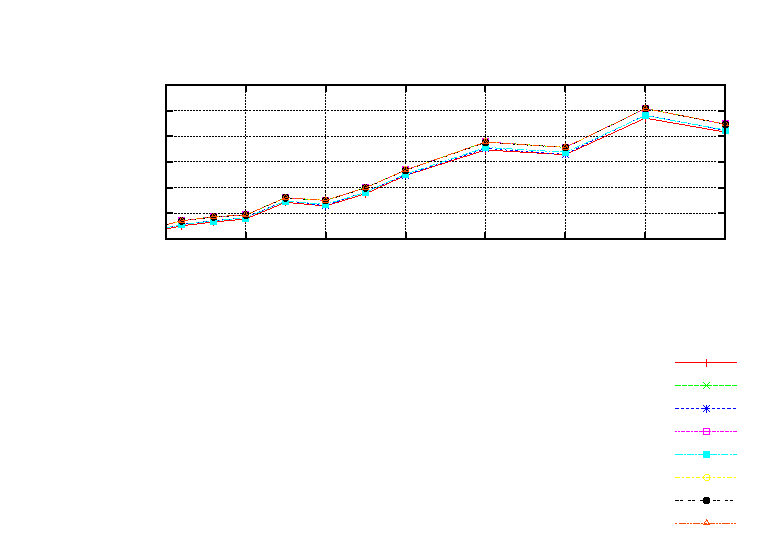
\includegraphics{ej3_frontera_connected_bipartite}}%
    \gplfronttext
  \end{picture}%
\endgroup
}
    \caption{Fronteras para grafos bipartitos}
\end{figure}

\bigskip

\par Para estas tres familias (circulares, estrellas y bipartitos) se observan los mismos
    resultados que para la familia de $Ruedas$ (cuya justificaci\'on te\'orica ya ha sido
    dada en la secci\'on anterior).

%Banana
\begin{figure}[H]
    \centering
    \fontsize{7}{10}\selectfont
    \resizebox{0.8\textwidth}{!}{% GNUPLOT: LaTeX picture with Postscript
\begingroup
  \makeatletter
  \providecommand\color[2][]{%
    \GenericError{(gnuplot) \space\space\space\@spaces}{%
      Package color not loaded in conjunction with
      terminal option `colourtext'%
    }{See the gnuplot documentation for explanation.%
    }{Either use 'blacktext' in gnuplot or load the package
      color.sty in LaTeX.}%
    \renewcommand\color[2][]{}%
  }%
  \providecommand\includegraphics[2][]{%
    \GenericError{(gnuplot) \space\space\space\@spaces}{%
      Package graphicx or graphics not loaded%
    }{See the gnuplot documentation for explanation.%
    }{The gnuplot epslatex terminal needs graphicx.sty or graphics.sty.}%
    \renewcommand\includegraphics[2][]{}%
  }%
  \providecommand\rotatebox[2]{#2}%
  \@ifundefined{ifGPcolor}{%
    \newif\ifGPcolor
    \GPcolortrue
  }{}%
  \@ifundefined{ifGPblacktext}{%
    \newif\ifGPblacktext
    \GPblacktexttrue
  }{}%
  % define a \g@addto@macro without @ in the name:
  \let\gplgaddtomacro\g@addto@macro
  % define empty templates for all commands taking text:
  \gdef\gplbacktext{}%
  \gdef\gplfronttext{}%
  \makeatother
  \ifGPblacktext
    % no textcolor at all
    \def\colorrgb#1{}%
    \def\colorgray#1{}%
  \else
    % gray or color?
    \ifGPcolor
      \def\colorrgb#1{\color[rgb]{#1}}%
      \def\colorgray#1{\color[gray]{#1}}%
      \expandafter\def\csname LTw\endcsname{\color{white}}%
      \expandafter\def\csname LTb\endcsname{\color{black}}%
      \expandafter\def\csname LTa\endcsname{\color{black}}%
      \expandafter\def\csname LT0\endcsname{\color[rgb]{1,0,0}}%
      \expandafter\def\csname LT1\endcsname{\color[rgb]{0,1,0}}%
      \expandafter\def\csname LT2\endcsname{\color[rgb]{0,0,1}}%
      \expandafter\def\csname LT3\endcsname{\color[rgb]{1,0,1}}%
      \expandafter\def\csname LT4\endcsname{\color[rgb]{0,1,1}}%
      \expandafter\def\csname LT5\endcsname{\color[rgb]{1,1,0}}%
      \expandafter\def\csname LT6\endcsname{\color[rgb]{0,0,0}}%
      \expandafter\def\csname LT7\endcsname{\color[rgb]{1,0.3,0}}%
      \expandafter\def\csname LT8\endcsname{\color[rgb]{0.5,0.5,0.5}}%
    \else
      % gray
      \def\colorrgb#1{\color{black}}%
      \def\colorgray#1{\color[gray]{#1}}%
      \expandafter\def\csname LTw\endcsname{\color{white}}%
      \expandafter\def\csname LTb\endcsname{\color{black}}%
      \expandafter\def\csname LTa\endcsname{\color{black}}%
      \expandafter\def\csname LT0\endcsname{\color{black}}%
      \expandafter\def\csname LT1\endcsname{\color{black}}%
      \expandafter\def\csname LT2\endcsname{\color{black}}%
      \expandafter\def\csname LT3\endcsname{\color{black}}%
      \expandafter\def\csname LT4\endcsname{\color{black}}%
      \expandafter\def\csname LT5\endcsname{\color{black}}%
      \expandafter\def\csname LT6\endcsname{\color{black}}%
      \expandafter\def\csname LT7\endcsname{\color{black}}%
      \expandafter\def\csname LT8\endcsname{\color{black}}%
    \fi
  \fi
  \setlength{\unitlength}{0.0500bp}%
  \begin{picture}(7200.00,5040.00)%
    \gplgaddtomacro\gplbacktext{%
      \csname LTb\endcsname%
      \put(1034,3124){\makebox(0,0)[r]{\strut{} 0}}%
      \csname LTb\endcsname%
      \put(1034,3333){\makebox(0,0)[r]{\strut{} 10}}%
      \csname LTb\endcsname%
      \put(1034,3542){\makebox(0,0)[r]{\strut{} 20}}%
      \csname LTb\endcsname%
      \put(1034,3752){\makebox(0,0)[r]{\strut{} 30}}%
      \csname LTb\endcsname%
      \put(1034,3961){\makebox(0,0)[r]{\strut{} 40}}%
      \csname LTb\endcsname%
      \put(1034,4170){\makebox(0,0)[r]{\strut{} 50}}%
      \csname LTb\endcsname%
      \put(1034,4379){\makebox(0,0)[r]{\strut{} 60}}%
      \csname LTb\endcsname%
      \put(1166,2904){\makebox(0,0){\strut{} 0}}%
      \csname LTb\endcsname%
      \put(1730,2904){\makebox(0,0){\strut{} 1000}}%
      \csname LTb\endcsname%
      \put(2293,2904){\makebox(0,0){\strut{} 2000}}%
      \csname LTb\endcsname%
      \put(2857,2904){\makebox(0,0){\strut{} 3000}}%
      \csname LTb\endcsname%
      \put(3421,2904){\makebox(0,0){\strut{} 4000}}%
      \csname LTb\endcsname%
      \put(3985,2904){\makebox(0,0){\strut{} 5000}}%
      \csname LTb\endcsname%
      \put(4548,2904){\makebox(0,0){\strut{} 6000}}%
      \csname LTb\endcsname%
      \put(5112,2904){\makebox(0,0){\strut{} 7000}}%
      \csname LTb\endcsname%
      \put(5676,2904){\makebox(0,0){\strut{} 8000}}%
      \csname LTb\endcsname%
      \put(6239,2904){\makebox(0,0){\strut{} 9000}}%
      \csname LTb\endcsname%
      \put(6803,2904){\makebox(0,0){\strut{} 10000}}%
      \put(176,3751){\rotatebox{-270}{\makebox(0,0){\strut{}Tiempo ($nanosegundos^{\sfrac{1}{5}}$)}}}%
      \put(396,3751){\rotatebox{-270}{\makebox(0,0){\strut{}(Escala Lineal)}}}%
      \put(3984,2574){\makebox(0,0){\strut{}Cantidad de Nodos}}%
      \put(3984,2354){\makebox(0,0){\strut{}(Escala Lineal)}}%
      \put(3984,4709){\makebox(0,0){\strut{}Tiempo de ejecución conforme aumenta la cantidad de nodos}}%
    }%
    \gplgaddtomacro\gplfronttext{%
      \csname LTb\endcsname%
      \put(6065,1933){\makebox(0,0)[r]{\strut{}Primer Vecino}}%
      \csname LTb\endcsname%
      \put(6065,1713){\makebox(0,0)[r]{\strut{}Primer Vecino con golosa}}%
      \csname LTb\endcsname%
      \put(6065,1493){\makebox(0,0)[r]{\strut{}Primer Vecino con intercambio}}%
      \csname LTb\endcsname%
      \put(6065,1273){\makebox(0,0)[r]{\strut{}Primer Vecino con intercambio y golosa}}%
      \csname LTb\endcsname%
      \put(6065,1053){\makebox(0,0)[r]{\strut{}Mejor Vecino}}%
      \csname LTb\endcsname%
      \put(6065,833){\makebox(0,0)[r]{\strut{}Mejor Vecino con golosa}}%
      \csname LTb\endcsname%
      \put(6065,613){\makebox(0,0)[r]{\strut{}Mejor Vecino con intercambio}}%
      \csname LTb\endcsname%
      \put(6065,393){\makebox(0,0)[r]{\strut{}Mejor Vecino con intercambio y golosa}}%
      \csname LTb\endcsname%
      \put(6065,173){\makebox(0,0)[r]{\strut{}Cota teórica superior $\mathcal O(n)$}}%
    }%
    \gplbacktext
    \put(0,0){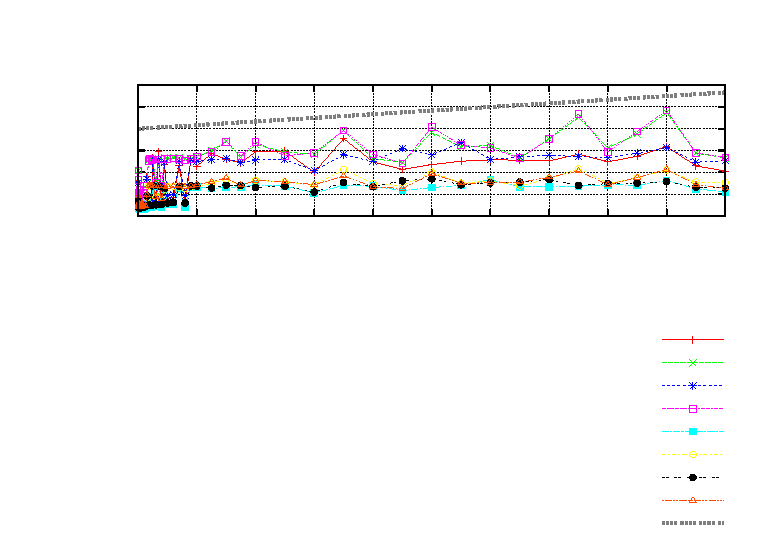
\includegraphics{ej3_nodos_banana}}%
    \gplfronttext
  \end{picture}%
\endgroup
}
    \caption{Complejidad temporal para grafos Banana Tree}
\end{figure}

\begin{figure}[H]
    \centering
    \fontsize{7}{10}\selectfont
    \resizebox{0.8\textwidth}{!}{% GNUPLOT: LaTeX picture with Postscript
\begingroup
  \makeatletter
  \providecommand\color[2][]{%
    \GenericError{(gnuplot) \space\space\space\@spaces}{%
      Package color not loaded in conjunction with
      terminal option `colourtext'%
    }{See the gnuplot documentation for explanation.%
    }{Either use 'blacktext' in gnuplot or load the package
      color.sty in LaTeX.}%
    \renewcommand\color[2][]{}%
  }%
  \providecommand\includegraphics[2][]{%
    \GenericError{(gnuplot) \space\space\space\@spaces}{%
      Package graphicx or graphics not loaded%
    }{See the gnuplot documentation for explanation.%
    }{The gnuplot epslatex terminal needs graphicx.sty or graphics.sty.}%
    \renewcommand\includegraphics[2][]{}%
  }%
  \providecommand\rotatebox[2]{#2}%
  \@ifundefined{ifGPcolor}{%
    \newif\ifGPcolor
    \GPcolortrue
  }{}%
  \@ifundefined{ifGPblacktext}{%
    \newif\ifGPblacktext
    \GPblacktexttrue
  }{}%
  % define a \g@addto@macro without @ in the name:
  \let\gplgaddtomacro\g@addto@macro
  % define empty templates for all commands taking text:
  \gdef\gplbacktext{}%
  \gdef\gplfronttext{}%
  \makeatother
  \ifGPblacktext
    % no textcolor at all
    \def\colorrgb#1{}%
    \def\colorgray#1{}%
  \else
    % gray or color?
    \ifGPcolor
      \def\colorrgb#1{\color[rgb]{#1}}%
      \def\colorgray#1{\color[gray]{#1}}%
      \expandafter\def\csname LTw\endcsname{\color{white}}%
      \expandafter\def\csname LTb\endcsname{\color{black}}%
      \expandafter\def\csname LTa\endcsname{\color{black}}%
      \expandafter\def\csname LT0\endcsname{\color[rgb]{1,0,0}}%
      \expandafter\def\csname LT1\endcsname{\color[rgb]{0,1,0}}%
      \expandafter\def\csname LT2\endcsname{\color[rgb]{0,0,1}}%
      \expandafter\def\csname LT3\endcsname{\color[rgb]{1,0,1}}%
      \expandafter\def\csname LT4\endcsname{\color[rgb]{0,1,1}}%
      \expandafter\def\csname LT5\endcsname{\color[rgb]{1,1,0}}%
      \expandafter\def\csname LT6\endcsname{\color[rgb]{0,0,0}}%
      \expandafter\def\csname LT7\endcsname{\color[rgb]{1,0.3,0}}%
      \expandafter\def\csname LT8\endcsname{\color[rgb]{0.5,0.5,0.5}}%
    \else
      % gray
      \def\colorrgb#1{\color{black}}%
      \def\colorgray#1{\color[gray]{#1}}%
      \expandafter\def\csname LTw\endcsname{\color{white}}%
      \expandafter\def\csname LTb\endcsname{\color{black}}%
      \expandafter\def\csname LTa\endcsname{\color{black}}%
      \expandafter\def\csname LT0\endcsname{\color{black}}%
      \expandafter\def\csname LT1\endcsname{\color{black}}%
      \expandafter\def\csname LT2\endcsname{\color{black}}%
      \expandafter\def\csname LT3\endcsname{\color{black}}%
      \expandafter\def\csname LT4\endcsname{\color{black}}%
      \expandafter\def\csname LT5\endcsname{\color{black}}%
      \expandafter\def\csname LT6\endcsname{\color{black}}%
      \expandafter\def\csname LT7\endcsname{\color{black}}%
      \expandafter\def\csname LT8\endcsname{\color{black}}%
    \fi
  \fi
  \setlength{\unitlength}{0.0500bp}%
  \begin{picture}(7200.00,5040.00)%
    \gplgaddtomacro\gplbacktext{%
      \csname LTb\endcsname%
      \put(1430,2904){\makebox(0,0)[r]{\strut{} 1}}%
      \csname LTb\endcsname%
      \put(1430,3273){\makebox(0,0)[r]{\strut{} 10}}%
      \csname LTb\endcsname%
      \put(1430,3642){\makebox(0,0)[r]{\strut{} 100}}%
      \csname LTb\endcsname%
      \put(1430,4010){\makebox(0,0)[r]{\strut{} 1000}}%
      \csname LTb\endcsname%
      \put(1430,4379){\makebox(0,0)[r]{\strut{} 10000}}%
      \csname LTb\endcsname%
      \put(1562,2684){\makebox(0,0){\strut{} 0}}%
      \csname LTb\endcsname%
      \put(2086,2684){\makebox(0,0){\strut{} 1000}}%
      \csname LTb\endcsname%
      \put(2610,2684){\makebox(0,0){\strut{} 2000}}%
      \csname LTb\endcsname%
      \put(3134,2684){\makebox(0,0){\strut{} 3000}}%
      \csname LTb\endcsname%
      \put(3658,2684){\makebox(0,0){\strut{} 4000}}%
      \csname LTb\endcsname%
      \put(4183,2684){\makebox(0,0){\strut{} 5000}}%
      \csname LTb\endcsname%
      \put(4707,2684){\makebox(0,0){\strut{} 6000}}%
      \csname LTb\endcsname%
      \put(5231,2684){\makebox(0,0){\strut{} 7000}}%
      \csname LTb\endcsname%
      \put(5755,2684){\makebox(0,0){\strut{} 8000}}%
      \csname LTb\endcsname%
      \put(6279,2684){\makebox(0,0){\strut{} 9000}}%
      \csname LTb\endcsname%
      \put(6803,2684){\makebox(0,0){\strut{} 10000}}%
      \put(176,3641){\rotatebox{-270}{\makebox(0,0){\strut{}Frontera}}}%
      \put(396,3641){\rotatebox{-270}{\makebox(0,0){\strut{}(Escala Logaritmica)}}}%
      \put(4182,2354){\makebox(0,0){\strut{}Cantidad de Nodos}}%
      \put(4182,2134){\makebox(0,0){\strut{}(Escala Lineal)}}%
      \put(4182,4709){\makebox(0,0){\strut{}Relacion Frontera/Nodos}}%
    }%
    \gplgaddtomacro\gplfronttext{%
      \csname LTb\endcsname%
      \put(6263,1713){\makebox(0,0)[r]{\strut{}Primer Vecino}}%
      \csname LTb\endcsname%
      \put(6263,1493){\makebox(0,0)[r]{\strut{}Primer Vecino con golosa}}%
      \csname LTb\endcsname%
      \put(6263,1273){\makebox(0,0)[r]{\strut{}Primer Vecino con intercambio}}%
      \csname LTb\endcsname%
      \put(6263,1053){\makebox(0,0)[r]{\strut{}Primer Vecino con intercambio y golosa}}%
      \csname LTb\endcsname%
      \put(6263,833){\makebox(0,0)[r]{\strut{}Mejor Vecino}}%
      \csname LTb\endcsname%
      \put(6263,613){\makebox(0,0)[r]{\strut{}Mejor Vecino con golosa}}%
      \csname LTb\endcsname%
      \put(6263,393){\makebox(0,0)[r]{\strut{}Mejor Vecino con intercambio}}%
      \csname LTb\endcsname%
      \put(6263,173){\makebox(0,0)[r]{\strut{}Mejor Vecino con intercambio y golosa}}%
    }%
    \gplbacktext
    \put(0,0){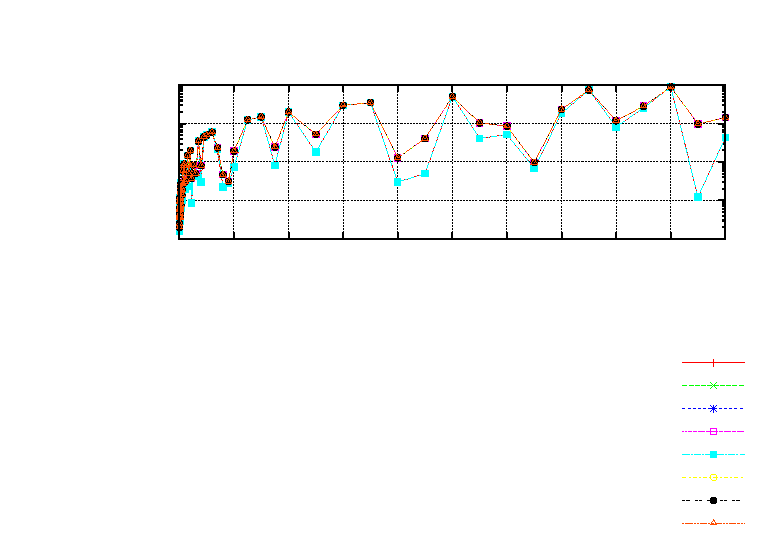
\includegraphics{ej3_frontera_banana}}%
    \gplfronttext
  \end{picture}%
\endgroup
}
    \caption{Fronteras para grafos Banana Tree}
\end{figure}

\par Para esta \'ultima familia, se observan resultados similares al de las \'ultimas
    familias exhibidas. En particular, la diferencia radica en la frontera devuelta
    por la variante ``Mejor Vecino''. Para el resto de las variantes se observa el
    mismo comportamiento (en cuanto a resultado obtenido), mientras que para esta
    variante mencionada se notan resultados de menor calidad. Nuevamente, por
    falta de tiempo, no se pudo investigar las causas de dicho comportamiento
    no esperado.

\subsubsection{Conclusiones}
\par Luego de observar los resultados de todas las variantes propuetas de nuestra
    heur\'istica, se observa cierto patr\'on para las familias de obtener
    mejores soluciones si se realizan saltos en la vecindad de mejor calida.

\par Dicha decisi\'on, en muchos casos, incluso conlleva a terminar la ejecuci\'on
    del programa m\'as r\'apidamente, contrario a lo que uno esperar\'ia. Esto
    se debe a que al dar saltos de mejor calidad, dichas variantes llegan a
    la soluci\'on de la heur\'istica m\'as r\'apido (no necesariamente la
    misma soluci\'on que las dem\'as variantes, pero en general se observ\'o
    que eran igual de buenas).

\par A\'un as\'i, cabe mencionar que existen casos donde dicha forma de recorrer
    la vecindad hace al algoritmo mucho m\'as ``lento'' que sus contrapartes.

\par Para finalizar, nos queda pendiente realizar una comparaci\'on de los
    resultados devueltos por esta heur\'istica, para poder as\'i verificar
    cuan buena es (respecto de las otras, al menos). Dicha comparaci\'on/experimentaci\'on
    se realiza en la Secci\'on~\ref{experimentacion}.
